\documentclass[article,shortnames]{jss}

%% -- LaTeX packages and custom commands ---------------------------------------

%% recommended packages
\usepackage{thumbpdf,lmodern}
\usepackage{amsmath, amsfonts}
\usepackage{bbm}% to get \mathbbmm{1}

%% another package (only for this demo article)
\usepackage{booktabs}
\usepackage{adjustbox}
\usepackage{tabularx}
\usepackage{rotating}

%% packages for the table
\usepackage{booktabs}
\usepackage{array}
\usepackage{pdflscape}
\usepackage{float}
\usepackage{longtable}
\usepackage{multirow}

\usepackage{xcolor}
\usepackage{colortbl}



%% new custom commands
\newcommand{\class}[1]{`\code{#1}'}
\newcommand{\fct}[1]{\code{#1()}}

%% For Sweave-based articles about R packages:
%% need no \usepackage{Sweave}



%% -- Article metainformation (author, title, ...) -----------------------------

%% - \author{} with primary affiliation
%% - \Plainauthor{} without affiliations
%% - Separate authors by \And or \AND (in \author) or by comma (in \Plainauthor).
%% - \AND starts a new line, \And does not.
\author{Nikos I. Bosse\\London School of Hygiene and Tropical Medicine
   \And Second Author\\Plus Affiliation}
\Plainauthor{Nikos I. Bosse, Second Author}

%% - \title{} in title case
%% - \Plaintitle{} without LaTeX markup (if any)
%% - \Shorttitle{} with LaTeX markup (if any), used as running title
\title{Evaluating Covid-19 Short-Term Forecasts using \pkg{scoringutils} in \proglang{R}}
\Plaintitle{Evaluating Covid-19 Short-Term Forecasts using scoringutils in R}
\Shorttitle{Evaluating Forecasts with \pkg{scoringutils} in \proglang{R}}

%% - \Abstract{} almost as usual
\Abstract{
  Forecasts play an important role in a variety of fields. Its role in informing public policy has attracted increased attention from the general public with the emergence of the Covid-19 pandemic. Evaluating forecasts, however, is not trivial in practice. Even though scoring methods such as proper scoring rules have been widely studied in the past, there is a lack of software implementation that allows a forecaster to conveniently evaluate their forecasts. In this paper we introduce \pkg{scoringutils}, an \proglang{R} package that facilitates automated forecast evaluation. It gives the user access to a wide range of scoring metrics for various types of forecasts as well as a variety of ways to visualise the evaluation. We give an overview of the evaluation process and the metrics implemented in \pkg{scoringutils} and show a full evaluation of a set of short-term forecasts of public health related targets made by SPI-M during the 2020 Covid-19 epidemic in the United Kingdom. 
}

%% - \Keywords{} with LaTeX markup, at least one required
%% - \Plainkeywords{} without LaTeX markup (if necessary)
%% - Should be comma-separated and in sentence case.
\Keywords{JSS, style guide, comma-separated, not capitalized, \proglang{R}}
\Plainkeywords{JSS, style guide, comma-separated, not capitalized, R}

%% - \Address{} of at least one author
%% - May contain multiple affiliations for each author
%%   (in extra lines, separated by \emph{and}\\).
%% - May contain multiple authors for the same affiliation
%%   (in the same first line, separated by comma).
\Address{
  Nikos Bosse\\
  Centre for Mathematical Modelling of Infectious Diseases\\
  London School of Hygiene and Tropical Medicine\\
  Keppel Street \\ 
  London WC1E 7HT \\
  E-mail: \email{nikos.bosse@lshtm.ac.uk}\\
  % URL: \url{https://eeecon.uibk.ac.at/~zeileis/}
}

\begin{document}



%% -- Introduction -------------------------------------------------------------

%% - In principle "as usual".
%% - But should typically have some discussion of both _software_ and _methods_.
%% - Use \proglang{}, \pkg{}, and \code{} markup throughout the manuscript.
%% - If such markup is in (sub)section titles, a plain text version has to be
%%   added as well.
%% - All software mentioned should be properly \cite-d.
%% - All abbreviations should be introduced.
%% - Unless the expansions of abbreviations are proper names (like "Journal
%%   of Statistical Software" above) they should be in sentence case (like
%%   "generalized linear models" below).

\section[Introduction]{Introduction}
Good forecasts are of great interest to decision makers in various fields like finance (), weather predictions or infectious disease modeling \citep{funkShorttermForecastsInform2020}. An integral part of assessing and improving their usefulness is forecast evaluation. For decades, researchers therefore have developed and refined an arsenal of techniques not only to forecast, but also to evaluate these forecasts (see e.g. \cite{bracherEvaluatingEpidemicForecasts2020a}, \cite{funkAssessingPerformanceRealtime2019}, \cite{gneitingProbabilisticForecastsCalibration2007}, and \cite{gneitingStrictlyProperScoring2007}). Yet even with this rich body of research available, implementing a complete forecast evaluation in \proglang{R} is not trivial. We therefore present the \pkg{scoringutils} package. The goal of the scoringuitls package is to facilitate the evaluation process and to allow even inexperienced users to perform a thorough evaluation of their forecasts. In this paper we give a quick introduction of the fundamental ideas behind forecast evaluation, explain the evaluation metrics implemented in \pkg{scoringutils} and present a full example evaluation of Covid-19 related short-term forecasts in the UK \citep{funkShorttermForecastsInform2020}. 

\subsection{Forecast types and forecast formats}

In its most general sense, a forecast is the forecaster’s stated belief about the future \citep{gneitingStrictlyProperScoring2007} that can come in many different forms. Quantitative forecasts are either point forecasts or probabilistic in nature and can make statements about continuous, discrete or binary outcome variables. Point forecasts only give one single number for the most likely outcome, but do not quantify the forecaster's uncertainty. This limits their usefulness, as a very certain forecast may, for example, warrant a very different course of actions than does a very uncertain one. Probabilistic forecasts, in contrast, by definition provide a full predictive distribution. This makes them much more useful in any applied setting, as we learn about the forecaster's uncertainty and their belief about all aspects of the underlying data-generating distribution (including e.g. skewness or the width of its tails). Probabilistic forecasts are therefore the focus of this paper as well as the \pkg{scoringutils} package. 

The predictive distribution of a probabilistic forecast can be represented in different ways with implications for the appropriate evaluation approach. For most forecasting problems, predictive distributions are not readily available in a closed form (and the \pkg{scoringutils} package therefore does not support scoring them directly). Instead, predictive distributions are often represented by a set of quantiles or predictive samples. Predictive samples require a lot of storage space and also come with a loss of precision that is especially pronounced in the tails of the predictive distribution, where quite a lot of samples are needed to accurately characterise the distribution. For that reason, often quantiles or central prediction intervals are reported instead [citation FORECAST HUBS]. For binary prediction targets, common in many classification problems, a probabilistic forecasts is represented by the probability that an outcome will come true. DO I NEED TO TALK ABOUT MULTINOMIAL CLASSIFICATION PROBLEMS? Table \ref{tab:forecast-types} summarises the different forecast types and formats. The general forecasting paradigm \cite{gneitingProbabilisticForecastsCalibration2007}, however, that guides the evaluation process is the same irrespective of the reporting format, even though specific scoring metrics differ. 

\begin{table}[h!]
\centering
\begin{longtable}[t]{>{\raggedright\arraybackslash}p{3.5cm}>{\raggedright\arraybackslash}p{2.5cm}>{\raggedright\arraybackslash}p{4.5cm}}
\toprule
\textbf{Forecast type} & \textbf{Target type} & \textbf{Representation of the predictive distribution}\\
\midrule
Point forecast & continuous \newline  integer \newline  binary & one single number for the predicted outcome\\
\cmidrule{1-3}\pagebreak[0]
 & continuous \newline  integer & predictive samples \newline   quantiles \newline   closed analytical form\\
\cmidrule{2-3}\nopagebreak
\multirow{-2}{3.5cm}{\raggedright\arraybackslash Probabilistic forecast} & binary & binary probabilities\\
\bottomrule
\end{longtable}\caption{\label{tab:forecast-types} Ssummary of the different forceast types and forecast formats}
\end{table}


\subsection{The forecasting paradigm}

Any forecaster should aim to minimise the difference between the predictive distribution $F$ and the unknown true data-generating distribution $G$ \citep{gneitingProbabilisticForecastsCalibration2007}. For an ideal forecast, we therefore have 
%
$$ F = G. $$
%
As we don't know the true data-generating distribution, we cannot assess the difference between the two distributions directly. \cite{gneitingProbabilisticForecastsCalibration2007} instead suggest to focus on two central aspects of the predictive distribution, calibration and sharpness. Calibration refers to the statistical consistency between the predictive distribution and the observations. A well calibrated forecast does not systematically deviate from the observed values. For an in-depth discussion of different ways in which a forecast can be miscalibrated, we refer to \cite{gneitingProbabilisticForecastsCalibration2007}. Sharpness is a feature of the forecast only and describes how concentrated the predictive distribution is, i.e. how precise the forecasts are. The general forecasting paradigm states that we should maximise sharpness of the predictive distribution subject to calibration. A model that made very precise forecasts would be at best useless if the forecasts were wrong most of the time. On the other hand, a model may be well calibrated, but not sharp enough to be useful. Take a weather forecast that would assign 30 percent rain probability for every single day. It may be well calibrated over the course of a year (it would be marginally calibrated according to \cite{gneitingProbabilisticForecastsCalibration2007}), but we would of course prefer a more precise forecast. Figure \ref{fig:forecast-paradigm} illustrates the concepts of calibration and sharpness. 

\begin{figure}[h]
\centering
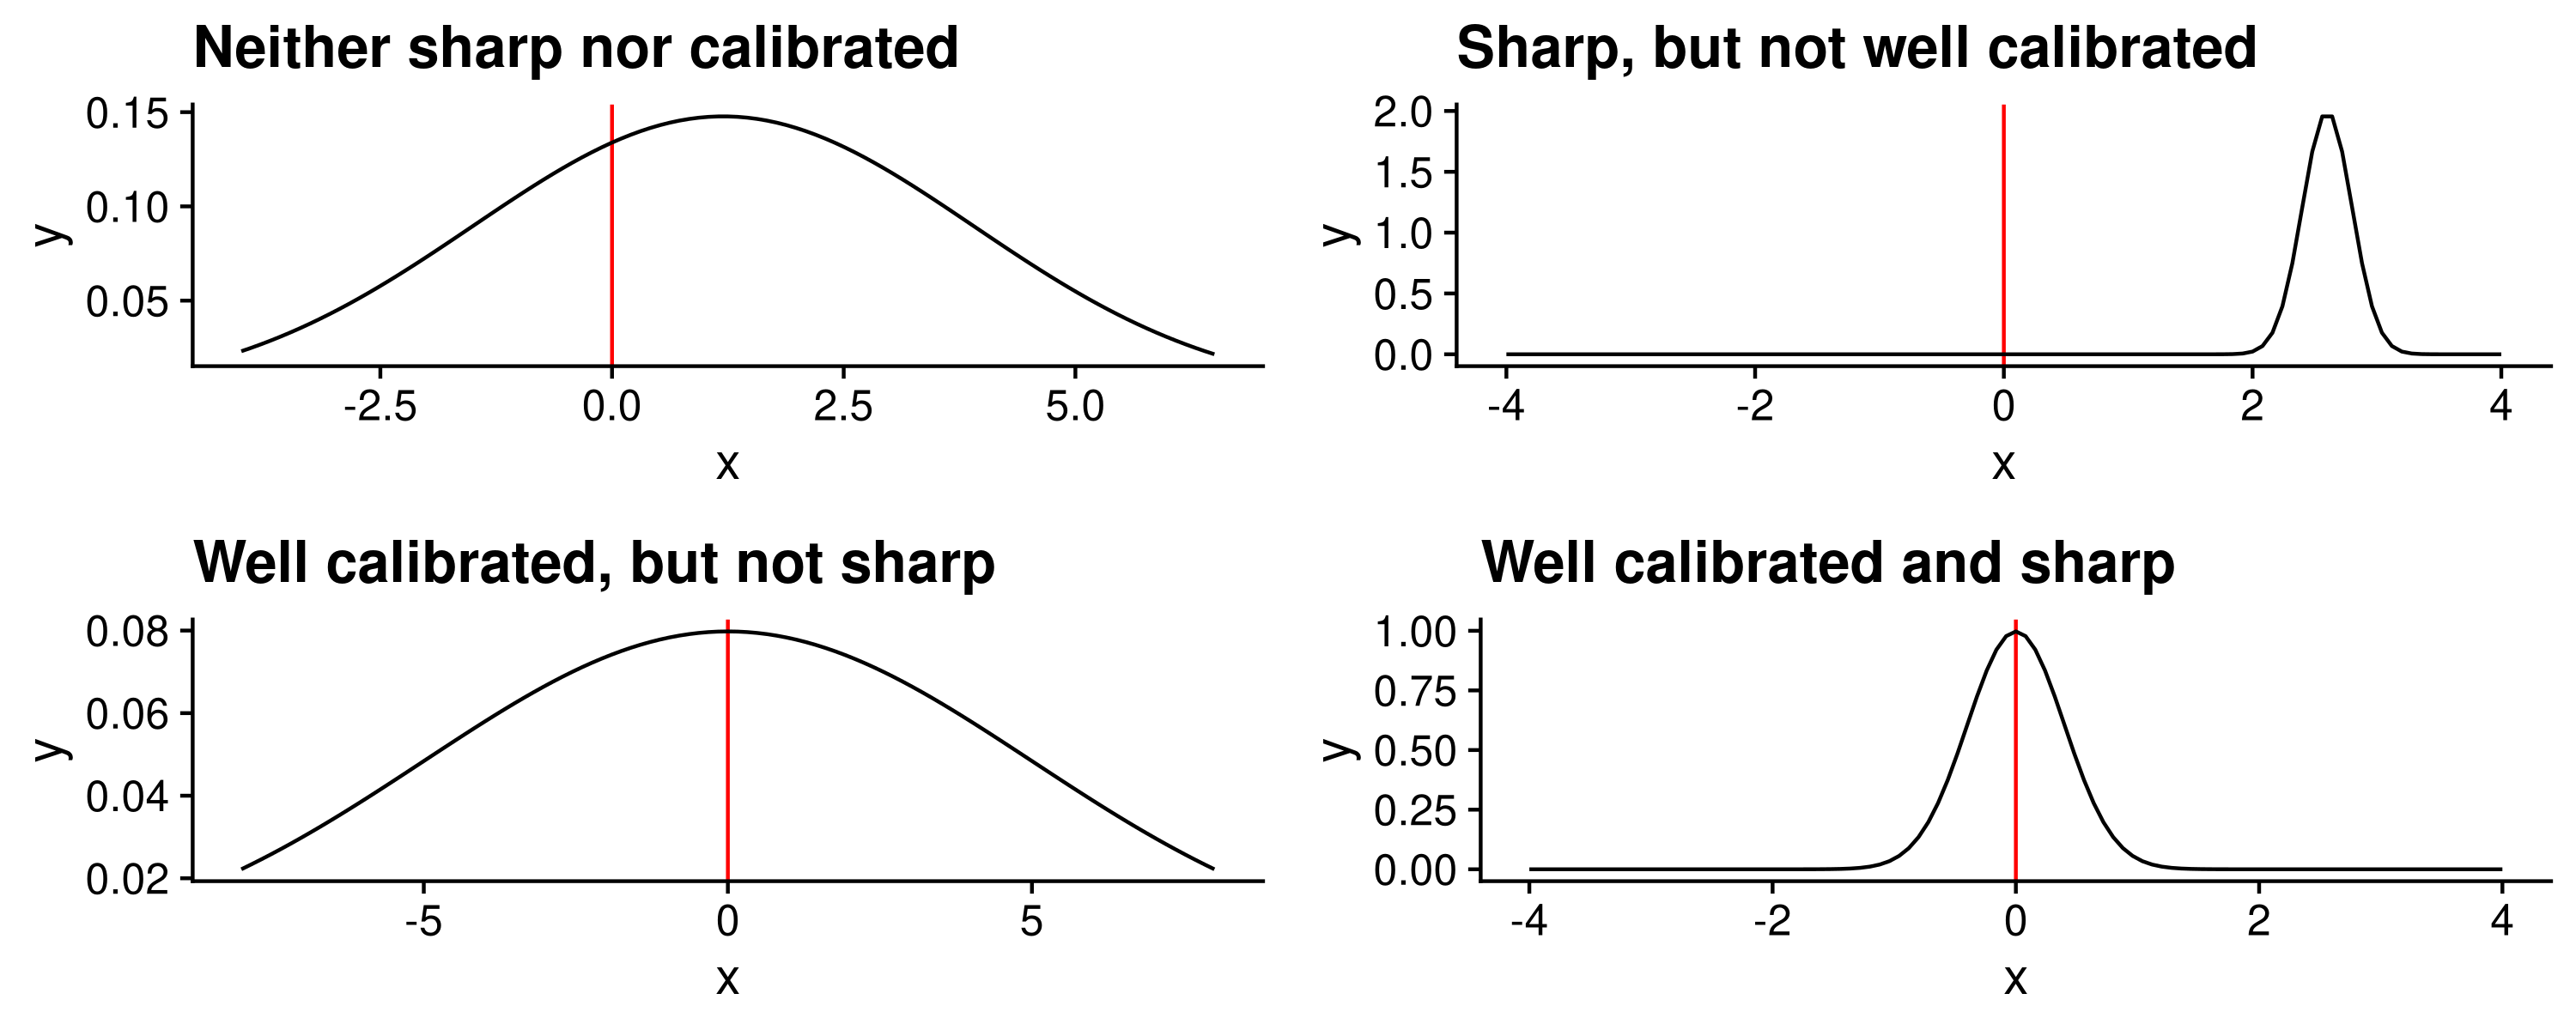
\includegraphics{plots/forecast-paradigm.png}
\caption{\label{fig:forecast-paradigm} Schematic illustration of calibration and sharpness. True value are represented in red, the predictive distribution is shown in black}
\end{figure}


% ==============================================================================
\section[metrics]{Scoring metrics implemented in \pkg{scoringutils}}

Some of the metrics in \pkg{scoringuitls} focus only on sharpness or on calibration. Others, called proper scoring rules, combine both aspects into a single number. The former can be helpful to learn about specific model aspects and improve them, the latter are especially useful to assess and rank predictive performance of a forecaster. The following gives an introduction to how these metrics can be used to evaluate forecasts. Table \ref{tab:table-summary-scores} shows an overview of the metrics implemented in \pkg{scoringutils}. Table \ref{tab:score-table} in the Appendix gives a thorough explanation of all the metrics. 

\begin{table}[h!]
\centering
\begin{longtable}[t]{>{\raggedright\arraybackslash}p{2.5cm}>{\raggedright\arraybackslash}p{2cm}>{\raggedright\arraybackslash}p{4.5cm}>{\raggedright\arraybackslash}p{4cm}}
\toprule
Metric & Target types & Forecast formats & Properties\\
\midrule
\endfirsthead
\multicolumn{4}{@{}l}{\textit{(continued)}}\\
\toprule
Metric & Target types & Forecast formats & Properties\\
\midrule
\endhead

\endfoot
\bottomrule
\endlastfoot
\cellcolor{gray!6}{CRPS (Continuous) ranked probability score} & \cellcolor{gray!6}{continuous, integer} & \cellcolor{gray!6}{closed-form, samples (approximation)} & \cellcolor{gray!6}{proper scoring rule, global, stable handling of outliers}\\
\addlinespace
Log score & continuous, (integer not in scoringutils) & closed-form, samples (approximation) & proper scoring rule, local, unstable for outliers\\
\addlinespace
\cellcolor{gray!6}{WIS (Weighted) interval score} & \cellcolor{gray!6}{continuous, integer} & \cellcolor{gray!6}{quantile or interval predictions} & \cellcolor{gray!6}{proper scoring rule, global, stable handling of outliers, converges to crps}\\
\addlinespace
DSS Dawid-Sebastiani score & continuous, integer & closed-form, samples (approximation) & proper scoring rule, somewhat global, somewhat stable handling of outliers\\
\addlinespace
\cellcolor{gray!6}{Brier score} & \cellcolor{gray!6}{binary} & \cellcolor{gray!6}{binary probabilities} & \cellcolor{gray!6}{proper scoring rule}\\
\addlinespace
Interval coverage & continuous, integer & interval forecasts (needs matching quantiles) & measure for calibration\\
\addlinespace
\cellcolor{gray!6}{Quantile coverage} & \cellcolor{gray!6}{continuous, integer} & \cellcolor{gray!6}{quantile or interval forecasts} & \cellcolor{gray!6}{measure for calibration}\\
\addlinespace
Probability integral transform (PIT) & continuous, integer, quantile & closed-form, samples, quantile or interval forecasts & assesses calibration\\
\addlinespace
\cellcolor{gray!6}{Sharpness} & \cellcolor{gray!6}{continuous, integer} & \cellcolor{gray!6}{closed-form, samples, quantile or interval forecasts} & \cellcolor{gray!6}{measures sharpness, slightly different depending on forecast format}\\
\addlinespace
Bias & continuous, integer, quantile & closed-form, samples, quantile or interval forecasts & captures tendency to over-or underpredict (aspect of calibration)\\
\addlinespace
\cellcolor{gray!6}{Mean score ratio} & \cellcolor{gray!6}{depends on score} & \cellcolor{gray!6}{depends on score} & \cellcolor{gray!6}{compares performance of two models}\\
\addlinespace
Relative skill & depends on scored & depends on score & Ranks models based on pairwise comparisons\\*
\end{longtable}\caption{\label{tab:table-summary-scores} Summary table of scores available in scoringutils}
\end{table}


\subsection{Proper scoring rules}

Proper scoring rules \citep{gneitingStrictlyProperScoring2007} jointly assess sharpness and calibration and assign a single numeric value to a forecast. A scoring rule is proper if a perfect forecaster (the predictive distribution equals the data-generating distribution) receives the lowest score on average. This makes sure that a forecaster evaluated by a proper scoring rule is always incentivised to state their best estimate. 

For sample-based forecasts, the (continuous) ranked probability score (crps) [CITATION], the log score (logs) [CITATION], and the Dawid-Sebastiani-score (dss) [CITATION] are available in \pkg{scoringutils}. These are implemented as wrappers around functions from the \pkg{scoringRules} package (which also has closed-form versions of the scoring rules available). They are in principle applicable to continuous as well as integer forecasts. The \pkg{scoringRules} implementation of the log score, however, requires a kernel density estimation that may be inappropriate for integer values (see also Table \ref{tab:table-summary-scores}) and is therefore not available for discrete predictions in \pkg{scoringutils}. 
For forecasts in an interval or quantile format, the weighted interval score (wis) \citep{bracherEvaluatingEpidemicForecasts2020a} is available. For an increasing number of equally-spaced prediction intervals, the wis converges to the crps and therefore has very similar properties. Binary forecasts can be scored using the Brier score (bs) [CITATION]. 

%sample-based proper scoring rules\usepackage{multirow}
When scoring forecasts in a sample-based format, the choice is usually between the log score and the crps. The dss is much less commonly used. It is easier to compute, but apart from that does not have immediate advantages over the former two. Crps and log score differ in two important aspects: the first is sensitivity to distance \cite{winklerScoringRulesEvaluation1996}, the second is how harshly far-off predictions are punished. 

The crps is a so-called global scoring rule, which means that the entire predictive distribution is taken into account when scoring a single forecast. The log score, on the other hand is local. The resulting score does not depend on the overall distance between the observed value and the distribution, but only on the probality density assigend to the actual outcome. Imagine two forecasters, A and B, who forecast the number of points scored in a basketball game. If both forecasters assigned the same probability to the true outcome (100 points), but A assigned higher probability to extreme outcomes far away from the actually observed outcome, then A will receive a worse score than B. The log score, in contrast, is a local scoring rule that only scores the probability assigned to the actual outcome and ignores the rest of the predictive distribution. Judged by the log score, A and B would receive exactly the same score. Sensitivity to distance (taking the entire predictive distribution into account) is arguably an advantage in most settings that involve decision making. Forecaster A's prediction that assigns high probability to results far away from the observed value is arguably less useful than B's forecast that assigns higher probability to values closer to it (the probability assigned to the actual outcome being equal for both forecasts). The log score is only implicitly sensitive to distance if we assume that values close to the observed value are actually more likely to occur. It may, however, be more appropriate for inferential purposes (see \cite{winklerScoringRulesEvaluation1996}). 

% stable vs. non-stable
A second important difference is how forecasts are treated that deviate strongly from the observered outcome. The crps can be thought of as a generalisation of the absolute error to a predictive distribution. It therefore scales linearly with the distance between forecast distribution and true value. The log score, however, is the log of the predictive density evaluated at the observed value. It can therfore quickly go to negative infinity if the probability assigned to the observed outcome is close to zero. The crps is therefore considered more stable than the log score. The behaviour of the dss is in between the two. Whether or not harsh punishment of bad predictions is desirable or not depends of course on the setting. \cite{bracherEvaluatingEpidemicForecasts2020a} exemplify that in practice there may indeed be substantial differences between how the crps and log score judge the same forecast. 

% properties of the WIS + decomposition
For quantile forecasts the wis is the best available option and can be understood as an approximation to the crps. One additional benefit of the wis is that it can easily be decomposed into three additive components: an uncertainty penalty (sharpness) for the width of a prediction interval and penalties for over- and underprediction (if a value falls outside of a prediction interval). This can be very helpful in diagnosing model problems. It may therefore even be useful to convert samples into quantiles and use the wis instead of the crps to make use of this decomposition for the purpose of model diagnostics. 
% fact that scores scale with the overall level of the prediction
Both crps and wis, as generalisations of the absolute value, suffer from the fact that overall scores depend on the order of magnitude of the quantity we try to forecast. It can therefore be difficult to compare forecasts for very different targets. One possibility to address this is the use of pairwise comparisons introduced later. In general, this is much less of a problem for the log score and the dss. IS IT ONE AT ALL? 

\subsection{Evaluating calibration and sharpness independently}

In addition to the proper scoring rules outlined above, \pkg{scoringutils} makes numerous metrics available to evaluate calibration and sharpness independently. This is especially helpful for model diagnostics. 

\subsubsection{Assessing calibration} 

Several strategies have been proposed to detect systematic deviations of the predictive distributions from the observations (see e.g. \cite{funkAssessingPerformanceRealtime2019}; \cite{gneitingProbabilisticForecastsCalibration2007}; \cite{gneitingStrictlyProperScoring2007}). Using \pkg{scoringutils}, we can look at three different aspects of calibration: bias, empirical coverage, and the probability integral transform (PIT). 

% Bias
Bias, i.e. systematic over- or underprediction, is a very common form of miscalibration which therefore deserves separate attention. The bias metric (with slightly different versions for the various forecast types and formats) captures a general tendency to over- and underpredict that is bound to be between minus one (underpredicton) and one (overprediction), where zero is ideal. It is derived by looking at how much of the probability mass of the predictive distribution is below or above the true observed value. For quantile forecasts we have second alternative approach available to assess over- and underprediction - by simply looking at the corresponding components of the weighted interval score. What is different between the over- and underprediction components and bias as described above is its sensitivity to outliers. The former are derived from absolute differences, while the latter is bound and rather captures a general tendency to be biased. 

% interval coverage and quantile coverage
Another way to look at calibration (precisely: probabilistic calibration in \cite{gneitingProbabilisticForecastsCalibration2007}) is to compare the proportion of observed values covered by different parts of the predictive distribution with the nominal coverage implied by the CDF of the distribution. This is most easily understood in the context of quantile forecasts, but can easily be transferred to sample-based continuous and integer forecasts as well. 
%
To assess empirical coverage at a certain interval range, we simply measure the proportion of true observed values that fall into corresponding range of the predictive distribution. If the 0.05, 0.25, 0.75, and 0.95 quantiles are given, then 50\% of the true values should fall between the 0.25 and 0.75 quantiles and 90\% should fall between the 0.05 and 0.95 quantiles. We can calculate and plot these values to inspect how well different parts of the forecast distribution are calibrated. 
%
To get an even more precise picture, we can also look at the percentage of true values below every single quantile of the predictive distribution. This allows to diagnose issues in the lower and upper tails of the prediction intervals separately. A similar way to visualise the same information is a PIT histogram. In order to conveniently assess deviations between the predictive distribution and the true data-generating distribution we can transform the observed values using the probability integral transformation (PIT) \citep{dawidPresentPositionPotential1984} (see more details in Table \ref{tab:score-table}). If both distributions are equal, the transformed values will follow a uniform distribution. A histogram of the transformed values can help to diagnose systematic differences between the predictions and the observed values. Figure \ref{fig:calibration-plots} exemplifies the characteristic shape of certain systematic deviations of the predicitve distribution from the true data-generating distribution. In the PIT histograms, bias leads to a triangular shape, overdispersion results in a hump shaped form and underdispersion in a U-shape. ADD INTERPRETATION FOR QUANTILE AND INTERVAL COVERAGE PLOTS HERE. 

\begin{figure}[h]
\centering
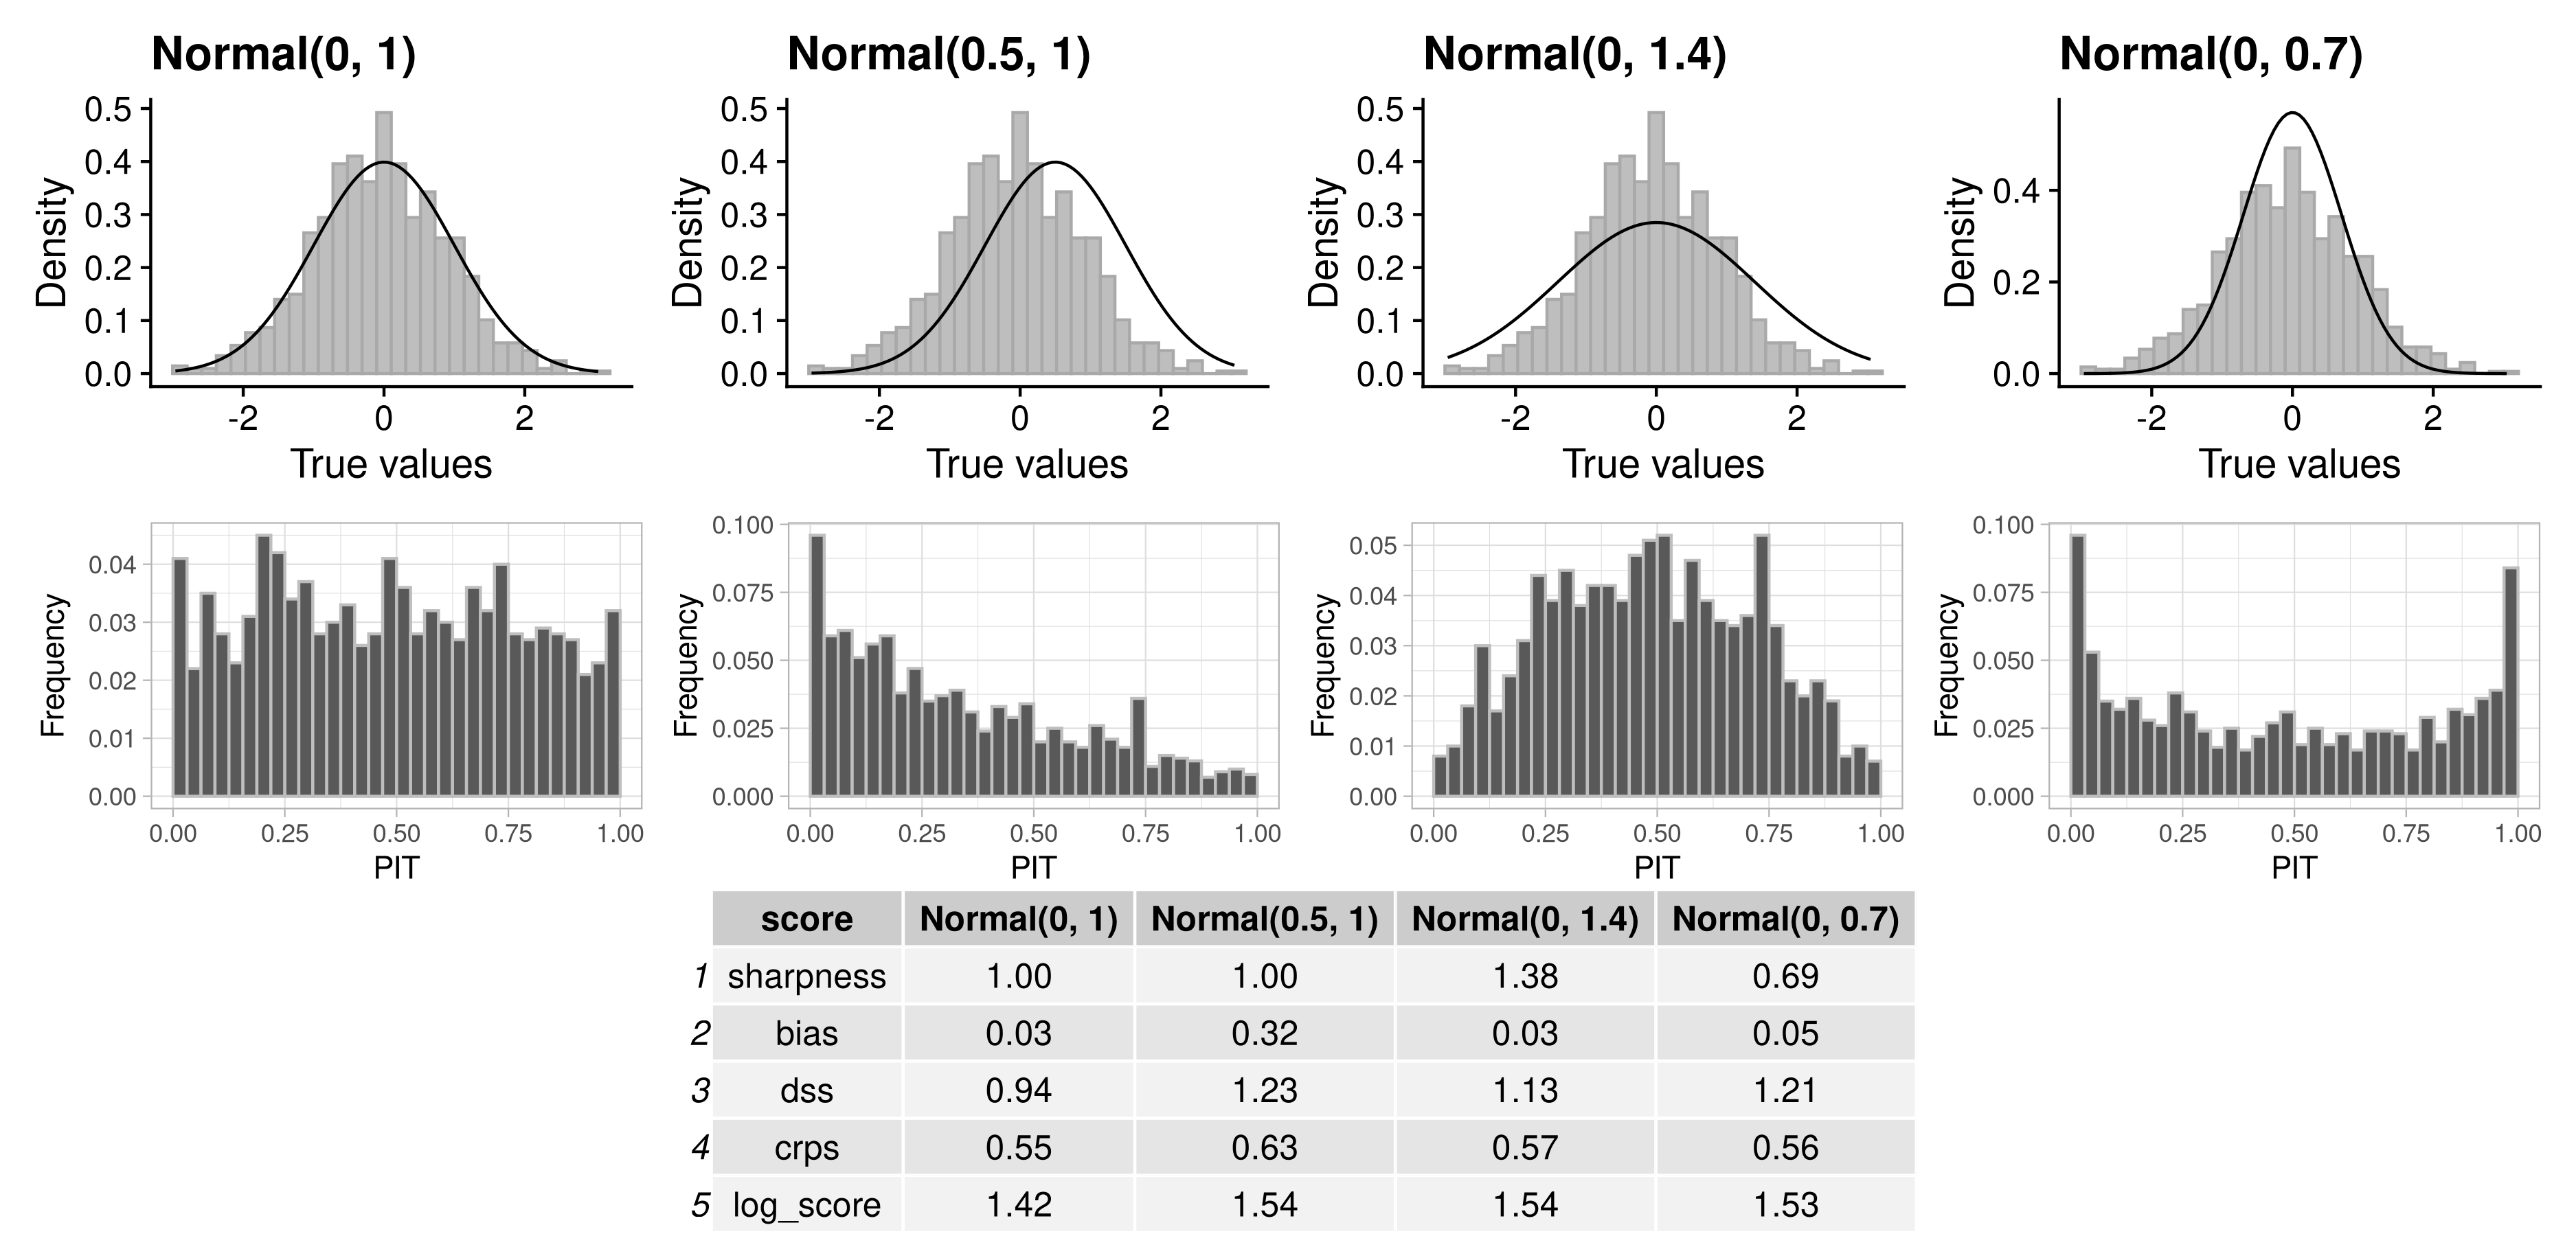
\includegraphics{plots/calibration-diagnostic-examples.png}
\caption{\label{fig:calibration-plots} Calibration plots for different forecast distributions. I plan to add interval and quantile coverage plots, but these still have to be made.}
\end{figure}




\subsubsection{Assessing sharpness}

Sharpness is the ability to produce narrow forecasts. It does not depend on the actual observations and is a quality of the forecast only \ref{gneitingProbabilisticForecastsCalibration2007}. Sharpness is therefore only useful subject to calibration, as exemplified above in Figure \ref{fig:calibration-example}. We may be willing to trade off a little calibration for a lot more sharpness, but usually not much. For sample-based forecasts, \pkg{scoringutils} calculates sharpness as the normalised median absolute deviation about the median (MADN) [funkAssessingPerformanceRealtime2019] (for details see Table \ref{tab:score-overview}). For quantile forecasts, we take the sharpness component of the wis which corresponds to a weighted average of the individual interval widths. 

WHAT WOULD BE REALLY COOL IS TO DETERMINE A WAY TO FIND THE OPTIMAL SHARPNESS OF A FORECAST. AS IS, I FEEL THIS PARAGRAPH IS SOMEWHAT USELESS. 

\subsection{Pairwise comparisons} 

If what we care about is to determine which model performs best, pairwise comparisons between models are a suitable approach [CITATION CRAMER et al.]. In turn, each pair of models is evaluated based on the targets that both models have predicted. The mean score by one model is divided by the mean score of the other model to obtain the mean score ratio (see Table \ref{tab:score-overview}, a measure of relative performance. To obtain an overall relative skill score for a model, we take the geomatric mean of all mean score ratios that involve that model  (omitting comparisons where there is no overlapping set of forecasts). This gives us an indicator of performance relative to all other models. The orientation depends on the score used. For the proper scoring rules described above, smaller is better and a relative skill score smaller than 1 indicates that a model is performing better than the average model. We can obtain a scaled relative skill score by dividing a model's relative skill by the relative skill of a baseline model. A scaled relative skill smaller than one then means that the model in question performed better than the baseline. 

It is in principle possible to obtain p-values that help determine whether two models perform significantly differently. \pkg{scoringutils} allows to compute these using eitab:score-tablether the Wilcoxon rank sum test or a permutation test. In practice, this is slightly complicated by the fact that both tests assume independent observations. In reality, however, forecasts by a model may be correlated across time or another dimension (e.g. if a forecaster has a bad day, they will likely perform badly across different targets for a given forecast date). P-values may therefore be too quick to suggest significant differences where there aren't any. One way to mitigate this is to aggregate observations over a category where one suspects correlation. A test that is performed on aggregate scores will likely be more conservative. 



% ==============================================================================
\section{Evaluating UK short-term forecasts}
\subsection{The data}

To illustrate the evaluation process with \pkg{scoringutils} we use short-term predictions of four different Covid-19 related targets in the UK made between March 31 and July 13 2020. Forecasts were produced by six groups in the UK, and submitted to the Scientific Pandemic Influenza Group on Modelling (SPI-M). The forecasts aimed to assess the likely future burden the UK healthcare system would face from the Covid-19 pandemic. Predictions were then aggregated and used to inform UK government health policy through the Strategic Advisory Group of Experts (SAGE). The data, as well as the individual forecast models are discussed in more depth in [FUNK ET AL]. 

- timing (weekly?) and number of forecast dates
- the four targets
- the models. 
- is the set complete?

We first need to obtain the data by installing and loading the \pkg{covid19.forecasts.uk} using the following commands: 
% 
\begin{Schunk}
\begin{Sinput}
R> # install and load data pacakge from external repository
R> # remotes::install_github("sbfnk/covid19.forecasts.uk")
R> 
R> # load packages
R> library(covid19.forecasts.uk)
R> library(dplyr)
R> library(scoringutils)
R> # load truth data
R> data(covid_uk_data)
R> # head(covid_uk_data)
R> 
R> # load forecasts
R> data(uk_forecasts)
R> # head(uk_forecasts)
\end{Sinput}
\end{Schunk}
% 
Let us take a first look a the data:
% 
\begin{Schunk}
\begin{Sinput}
R> glimpse(covid_uk_data)
\end{Sinput}
\begin{Soutput}
Rows: 4,174
Columns: 6
$ geography  <fct> London, London, London, London, London, London, L…
$ value_type <fct> hospital_inc, hospital_inc, hospital_inc, hospita…
$ value_desc <fct> Hospital admissions, Hospital admissions, Hospita…
$ truncation <dbl> 0, 0, 0, 0, 0, 0, 0, 0, 0, 0, 0, 0, 0, 0, 0, 0, 0…
$ value_date <date> 2020-03-20, 2020-03-21, 2020-03-22, 2020-03-23, …
$ value      <dbl> 18, 232, 280, 241, 313, 353, 516, 637, 677, 546, …
\end{Soutput}
\begin{Sinput}
R> glimpse(uk_forecasts)
\end{Sinput}
\begin{Soutput}
Rows: 1,254,513
Columns: 8
$ model         <fct> EpiSoon, EpiSoon, EpiSoon, EpiSoon, EpiSoon, E…
$ geography     <chr> "East of England", "East of England", "East of…
$ value_type    <fct> hospital_inc, hospital_inc, hospital_inc, hosp…
$ creation_date <date> 2020-03-31, 2020-03-31, 2020-03-31, 2020-03-3…
$ value_date    <date> 2020-04-01, 2020-04-02, 2020-04-03, 2020-04-0…
$ quantile      <dbl> 0.05, 0.05, 0.05, 0.05, 0.05, 0.05, 0.05, 0.05…
$ value         <dbl> 70, 64, 53, 42, 30, 19, 4, 0, 0, 0, 0, 0, 0, 0…
$ value_desc    <fct> Hospital admissions, Hospital admissions, Hosp…
\end{Soutput}
\end{Schunk}
% 
To bring the forecasts into the format needed for the evaluation, some minor changes need to be made to the data. The names of the columns that hold the forecasts and the true observed values need to be changed to \code{prediction} and \code{true_value}. While we could also proceed with separate data sets for the evaluation, we merge the two data sets in order to remove all instances where the forecasts, but not the true observations were made public. The \pkg{scoringutils} package provides a function that attempts to merge the data sets in a sensible way. 
% 
\begin{Schunk}
\begin{Sinput}
R> uk_forecasts <- rename(uk_forecasts, prediction = value)
R> covid_uk_data <-rename(covid_uk_data, true_value = value)
R> combined <- merge_pred_and_obs(uk_forecasts, covid_uk_data)
\end{Sinput}
\end{Schunk}
% 
Before we start with scoring the forecasts, it makes sense to start the evaluation process by visualising the data. To get a feeling for how complete the data set is, we can run the following code to obtain a heatmap with the number of available forecasts: 
% 
\begin{figure}[h]
\centering
\begin{Schunk}
\begin{Sinput}
R> show_avail_forecasts(combined, 
+                       x = "creation_date", 
+                       show_numbers = FALSE,
+                       legend_position = "bottom",
+                       facet_formula = ~ value_desc)
\end{Sinput}
\end{Schunk}
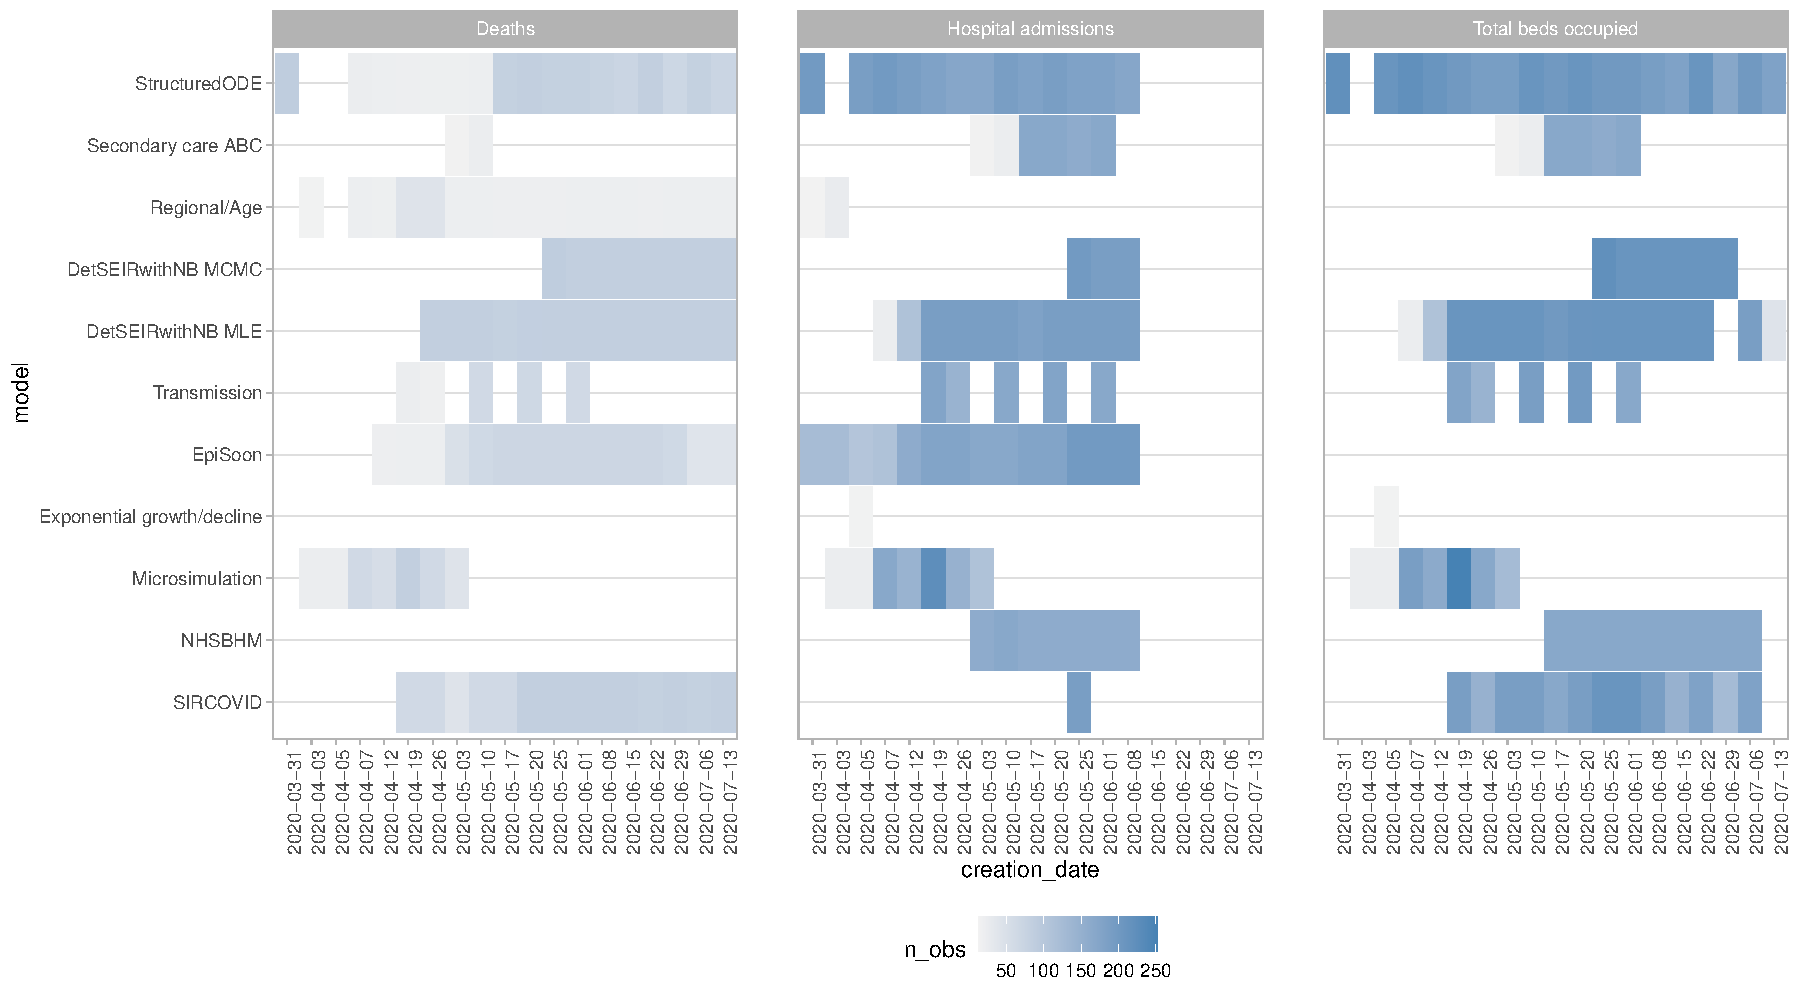
\includegraphics{plots/plot-show-availability}
\caption{\label{fig:avail-forecasts} Overview of the number of forecasts available}
\end{figure}
%THINK ABOUT WHETHER THIS FUNCTION CAN BE COMBINED WITH THE OTHER HEATMAP FUNCTION. 
% 
Missing forecasts can have a large impact on the forecast evaluation, if forecasts are not missing at random, but instead missingness correlates with performance. By default, the function treats a set of different quantiles or samples as one forecast. However, the user can specify manually which elements to treat as one forecast and which categories to sum over to count the number of available forecasts. 

Forecasts can be visualised using the \fct{plot\_predictions} function. The function accepts either a single combined data set or two separate truth data sets that can be merged together. Forecasts and observed values can be filtered independently, to show for example only predictions from a certain model or a specific number of weeks of true data before the forecast. Conditions to filter on need to be provided as a list of strings, where each of the strings represents an expression that can be evaluated to filter the data. To obtain, for example, a specific forecast from a model we are interest in, we can call: 
% 
\begin{figure}[h!]
\centering
\begin{Schunk}
\begin{Sinput}
R> locations <- 'c("Scotland", "Wales", "Northern Ireland", "England")'
R> plot_predictions(truth = covid_uk_data,
+                   forecasts = uk_forecasts,
+                   filter_both = list(paste("geography %in%", locations, collapse = "")),
+                   filter_truth = list('value_date <= "2020-06-22"',
+                                       'value_date > "2020-06-01"'), 
+                   filter_forecasts = list('model == "SIRCOVID"', 
+                                           'creation_date == "2020-06-22"'),
+                   x = "value_date",
+                   facet_formula = geography ~ value_type) + 
+    ggplot2::theme(legend.position = "bottom")
\end{Sinput}
\end{Schunk}
\caption{\label{fig:forecast-visualisation} Short-term forecasts made by the SIRCOVID model on June 22 2020.}
\end{figure}
% 
The output is shown in Figure \ref{fig:forecast-visualisation}.

\subsection[Scoring forecasts with eval_forecasts]{Scoring forecasts with \fct{eval\_forecasts}}

A full evaluation of all forecasts based on observed values can be performed using the function \fct{eval\_forecasts}. This requires a \code{data.frame} or similar which has at least a column called "prediction" and one called "true\_value". Depending on the exact input format, additional columns like "sample", "quantile", or "range" and "boundary" are needed. Additional columns may be present to indicate a grouping of forecasts, for example forecasts made in different locations or over different forecast horizons. We will not discuss all possible input formats here, but instead refer to the example data for each format that is provided with the package. Where possible, \pkg{scoringutils} also provides functionality to transform between various formats, e.g. from a sample based format to a quantile format. The \fct{eval\_forecasts} function automatically recognises the prediction type and input format, applies the appropriate scoring metrics and aggregates results as desired by the user. Internally, operations are handled using \pkg{data.table} to allow for fast and efficient computation.

As a first start for the evaluation of UK short-term forecasts, it makes sense to look at the scores achieved by every model separate for all prediction targets. This can be achieved by calling
% ion G
\begin{Schunk}
\begin{Sinput}
R> scores <- eval_forecasts(combined, 
+                           summarise_by = c("model", "value_desc"))
R> glimpse(scores)
\end{Sinput}
\begin{Soutput}
Rows: 29
Columns: 9
$ model              <fct> EpiSoon, StructuredODE, Microsimulation, …
$ value_desc         <fct> Hospital admissions, Hospital admissions,…
$ interval_score     <dbl> 38.56510, 61.75914, 100.71914, 35.44876, …
$ sharpness          <dbl> 22.886153, 6.133974, 33.985553, 10.365082…
$ underprediction    <dbl> 3.66782766, 24.82255866, 33.12350598, 8.5…
$ overprediction     <dbl> 12.0111222, 30.8026045, 33.6100814, 16.55…
$ coverage_deviation <dbl> 0.034531405, -0.268749094, -0.095652174, …
$ bias               <dbl> 0.26194170, -0.27368253, -0.39217045, -0.…
$ aem                <dbl> 45.96333, 73.38096, 138.14395, 53.22563, …
\end{Soutput}
\end{Schunk}
% 
If a more detailed analysis is desired, the level of aggregation can of course be changed to show for example separate scores for the different locations as well. This can be achieved using the \code{summarise_by} argument. To additionally stratify by location, we could specify \code{summarise_by = c("mode", "value_type", "geography")}. If we wanted to have one score per quantile or one per prediction interval range, we could specify something like \code{summarise_by = c("model", "quantile")} or \code{summarise_by = c("model", "quantile", "range")}. This can be useful if we, for example, want to analyse what proportion of true values are covered by certain interval ranges, or if we want to analyse the accuracy of the tails of the forecasts. When aggregating, \fct{eval\_forecasts} takes the mean according to the group defined in \code{summarise_by}. In the above example, if \code{summarise_by = c("model", "value_type")}, then scores would be averaged over all creation dates, forecast horizons (as represented by the the value dates), locations and quantiles to yield one score per model and forecast target. In addition to the mean, we can also obtain the standard deviation of the scores over which we average, as well as any desired quantile, by specifying \code{sd = TRUE} and for example \code{quantiles = c(0.5)} for the median. 

The user must, however, still exercise some caution when aggregating scores, as many of the metrics are absolute and scale with the magnitude of the quantity to forecast. Looking at one score per model (i.e. specifying \code{summarise_by = c("model")}) may not be so useful in this instance, as overall aggregate scores would be dominated by hospital admissions, while errors on death forecasts would have little influence. 

In the above example, we did not have to explicitly specify the \code{by} argument, but this may be necessary if additional columns are present in the data that do not indicate a grouping of forecasts. The \code{by} argument must then be used to denote the unit of a single forecast. In the above example, the unit of a single forecast would be \code{by = c("model", "geography", "value_type", "creation_date", "value_date", "value_desc")}. Quantiles should not be included, as several quantiles make up one forecast (and similarly for samples). If we had additional columns that do not serve to group forecasts (like for example the number of inhabitants in a certain location over time), these should also not be included. By default, if \code{by = NULL}, \fct{eval\_forecasts} will automatically use all present columns to determine the unit of a single forecast.

\subsection{Pairwise comparisons}

Pairwise comparisons between models [CITATION] can be obtained in two different ways. First, relative skill scores based on pairwise comparisons are by default returned from \fct{eval\_forecasts}. These will be computed separately for the categories defined in the \code{summarise_by} argument (excluding the category 'model'). Alternatively, a set of scores can be post-processed using the separate function \fct{pairwise\_comparison}. This approach is to be used for visualisation and if p-values for the pairwise comparisons are needed, as those are not returned from \fct{eval\_forecasts}. Usually, one would compute scores without specifying a \code{summarise_by} argument, but sometimes it may be sensible to average over certain scores, for example for predictions generated at a certain date. This allows to reduce the correlation between observations that enter the computation of p-values, which in turn makes the test less liberal. 
Using the function \fct{plot\_pairwise\_comparison} we can visualise the mean score ratios between all models as well as the 

\begin{Schunk}
\begin{Sinput}
R> # unsummarised scores
R> unsummarised_scores <- eval_forecasts(combined)
R> pairwise <- pairwise_comparison(unsummarised_scores, 
+                                  summarise_by = "value_desc")
\end{Sinput}
\end{Schunk}

The result is a \code{data.table} with different scores and metrics in a tidy format that can easily be used for further manipulation and plotting. 

\section{Visualisation and interpretation of evaluation results}

\subsection{Visualising aggregate scores and rankings}
A good starting point for an evaluation is the following score table that visusalises the scores we produced above. We can facet the table to account for the different forecast targets: 

\begin{figure}[h]
\centering
\begin{Schunk}
\begin{Sinput}
R> score_table(scores, y = "model", facet_formula = ~ value_desc)
\end{Sinput}
\end{Schunk}
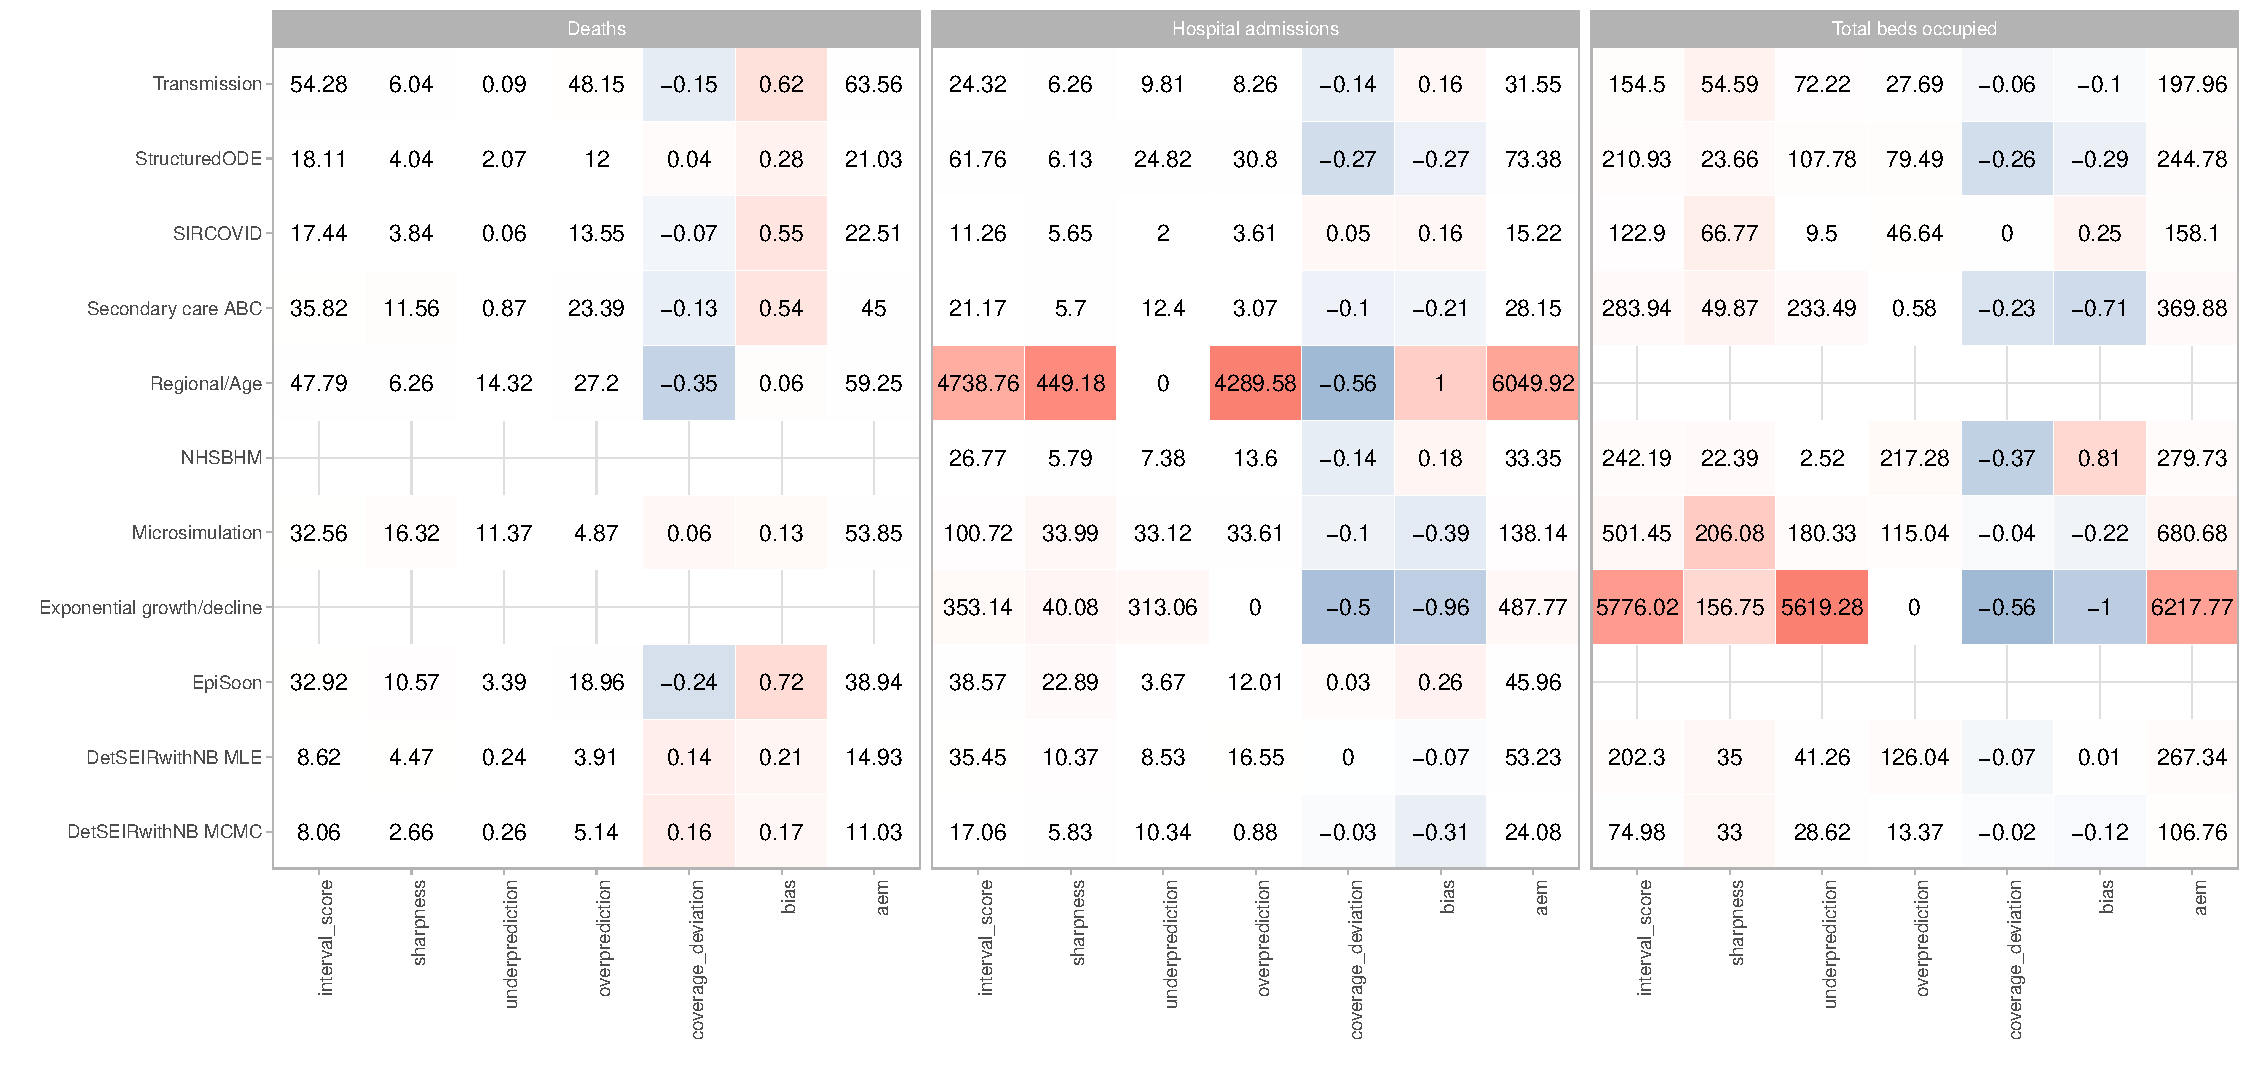
\includegraphics{plots/plot-score-table}
\caption{\label{fig:score-table} Coloured table to visualise the computed scores}
\end{figure}

The most informative metric in terms of model ranking is the relative\_skill. However, interpretation is not always straightforward and has to be done carefully. We can see that performance varied quite a bit across different metrics, where some models did well on one target, but poorly on another. Especially the Exponential growth/decline model stands out as it received the lowest relative skill score for hospital admissions, but the highest for the total number of beds occupied. Looking back at Figure \ref{fig:avail-forecasts}, we see that the model has only submitted very few forecasts over all. It may therefore be sensible to require all models to have submitted forecasts for at least 50\% of all forecast targets in order to enter the pairwise comparisons. For similar reasons, the interval score may be deceiving if looked at in isolation. As can be seen, the DetSEIRwithNB MLE model received a lower relative skill score, but a higher interval score than the DetSEIRwithNB MCMC model. This, again, can be explained by the fact that they forecasted different targets. The interval score, as an absolute metric, is highly influenced by the absolute value of the quantity that is forecasted. For the same reason, one should be careful when summarising interval scores from different locations or forecast targets, as the average score will be dominated by outliers as well as differences in the absolute level. Assuming a large enough set of available overlapping forecasts, the relative skill score is more robust. It therefore is reasonable to assume that the DetSEIRwithNB MLE forecasted quantities with a higher absolute value, but tended to perform worse than the DetSEIRwithNB MCMC model as far as we can tell based on the set of all pariwise comparisons. This can be confirmed for the direct comparison between the two by looking at the mean score ratios from the pairwise comparisons. These can be obtained by calling

\begin{figure}[h!]
\centering
\begin{Schunk}
\begin{Sinput}
R> plot_pairwise_comparison(pairwise) +
+    ggplot2::facet_wrap(~ value_desc, scales = "free_x") 
\end{Sinput}
\end{Schunk}
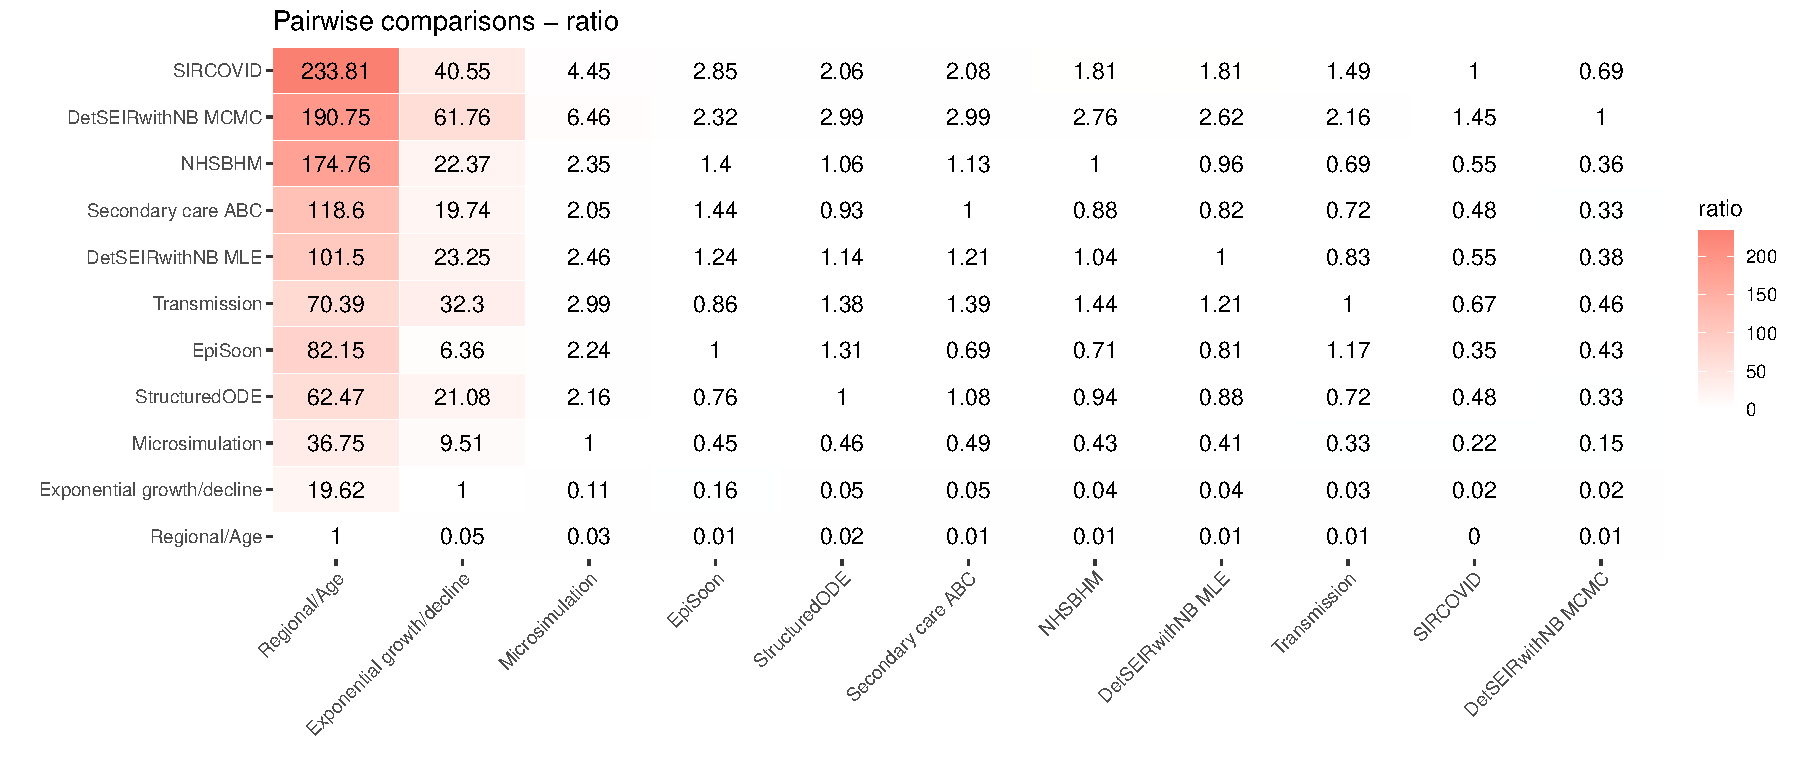
\includegraphics{plots/plot-pairwise-plot}
\caption{\label{fig:pairwise-comparison} Ratios of mean scores based on overlapping forecast sets. If a tile is blue, then the model on the y-axis performed better. If it is red, the model on the x-axis performed better in direct comparison. }
\end{figure}

we can also look at p-values in Figure \ref{fig:pairwise-comparison-pval} PROBABLY REMOVE THAT FROM THE PAPER
\begin{figure}[h!]
\centering
\begin{Schunk}
\begin{Sinput}
R> plot_pairwise_comparison(pairwise, type = "pval") +
+    ggplot2::facet_wrap(~ value_desc, scales = "free_x") 
\end{Sinput}
\end{Schunk}
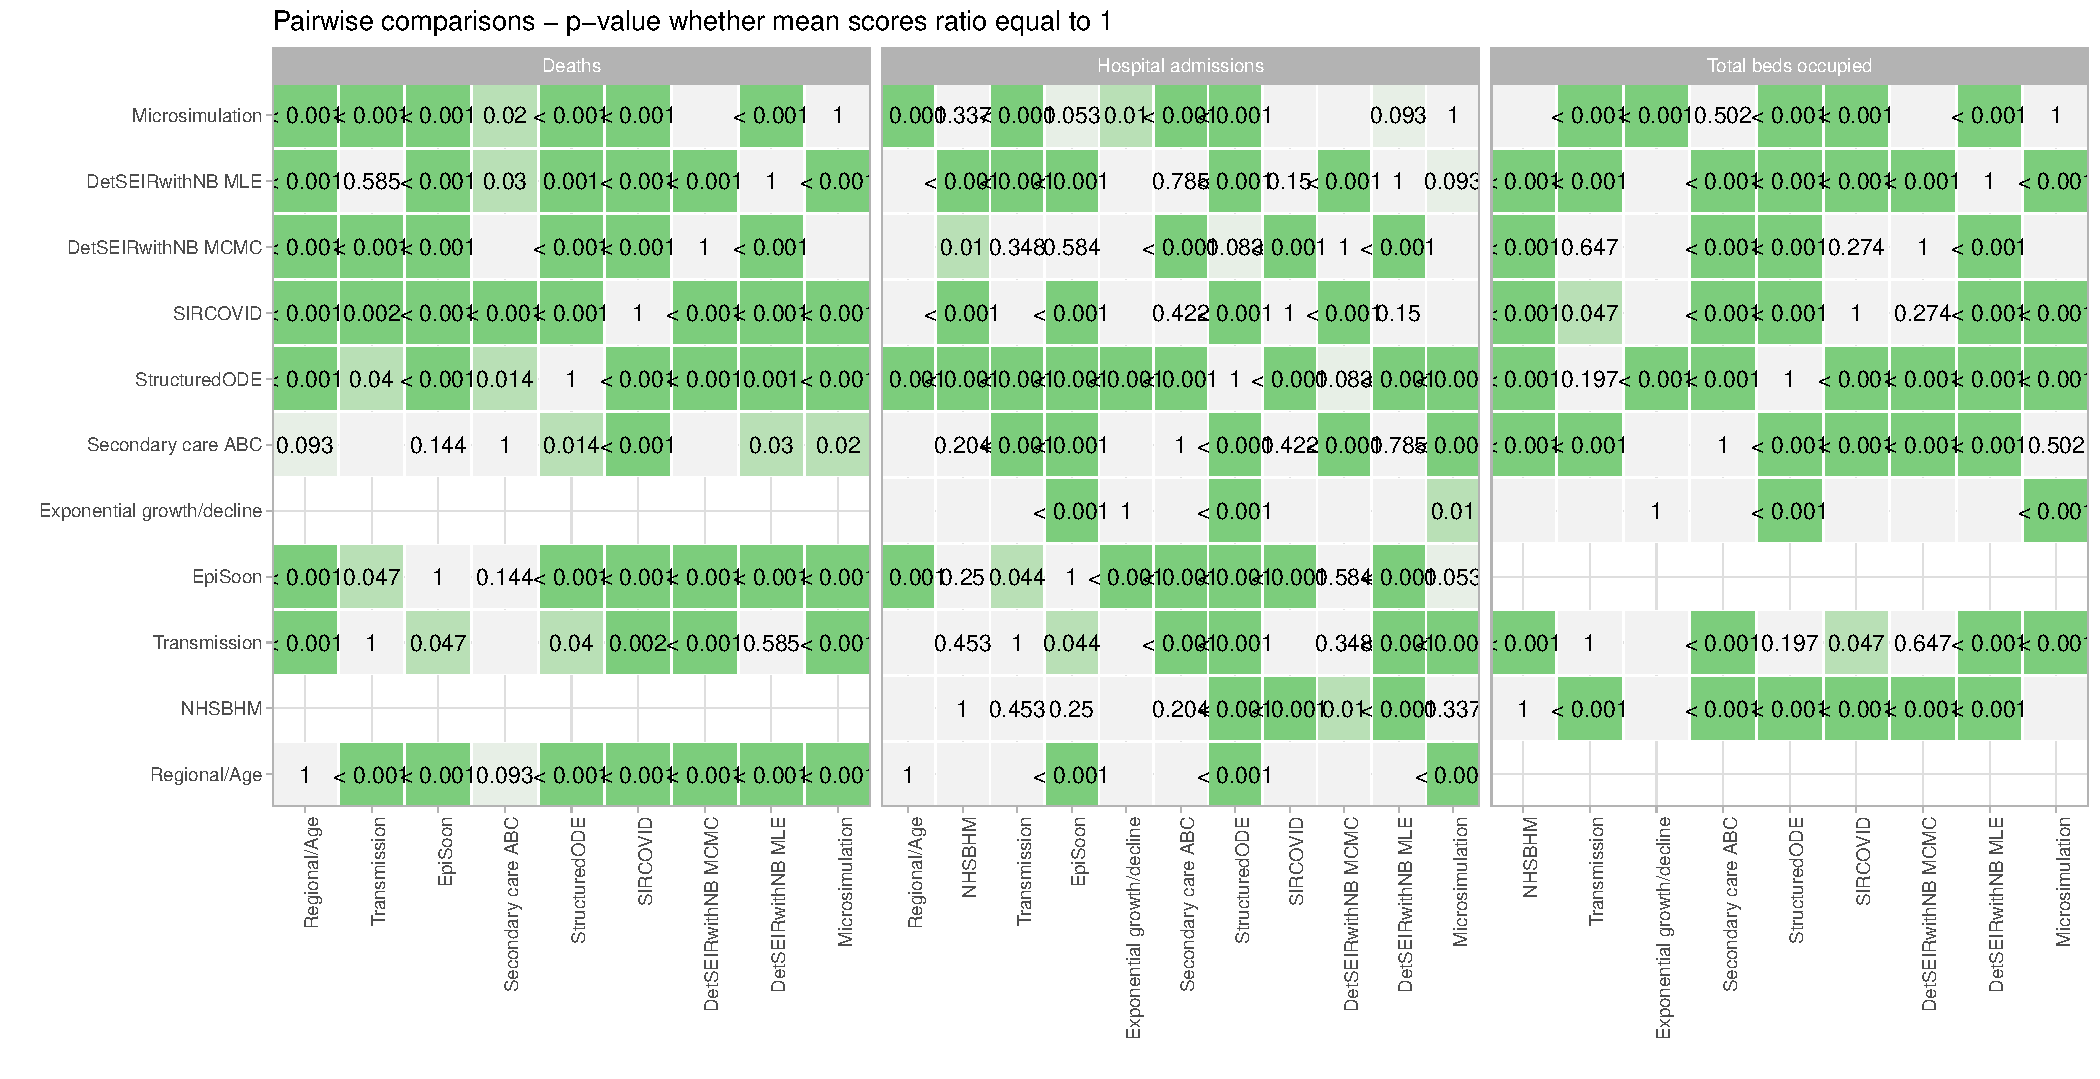
\includegraphics{plots/plot-pairwise-plot-ratio}
\caption{\label{fig:pairwise-comparison-pval} XXXX}
\end{figure}

In terms of actually understanding \textit{why} one model performs well or badly, the other metrics shown in Figure \ref{fig:score-table} provide additional insight. We turn to them in the following. 

\subsection{Visual model diagnostics}

For forecasts in an interval format, looking at the components of the weighted interval score separately is a natural next step. We can see in Figure \ref{fig:wis-components} that the majority of penalties come from over-and underprediction, instead of the sharpness component. We also see that most models tended to either over- or underpredict actual numbers.  

\begin{figure}[h!]
\centering
\begin{Schunk}
\begin{Sinput}
R> wis_components(scores, 
+                 facet_formula = ~ value_desc, 
+                 scales = "free_x") + 
+    ggplot2::coord_flip() + 
+    ggplot2::theme(legend.position = "bottom")
\end{Sinput}
\end{Schunk}
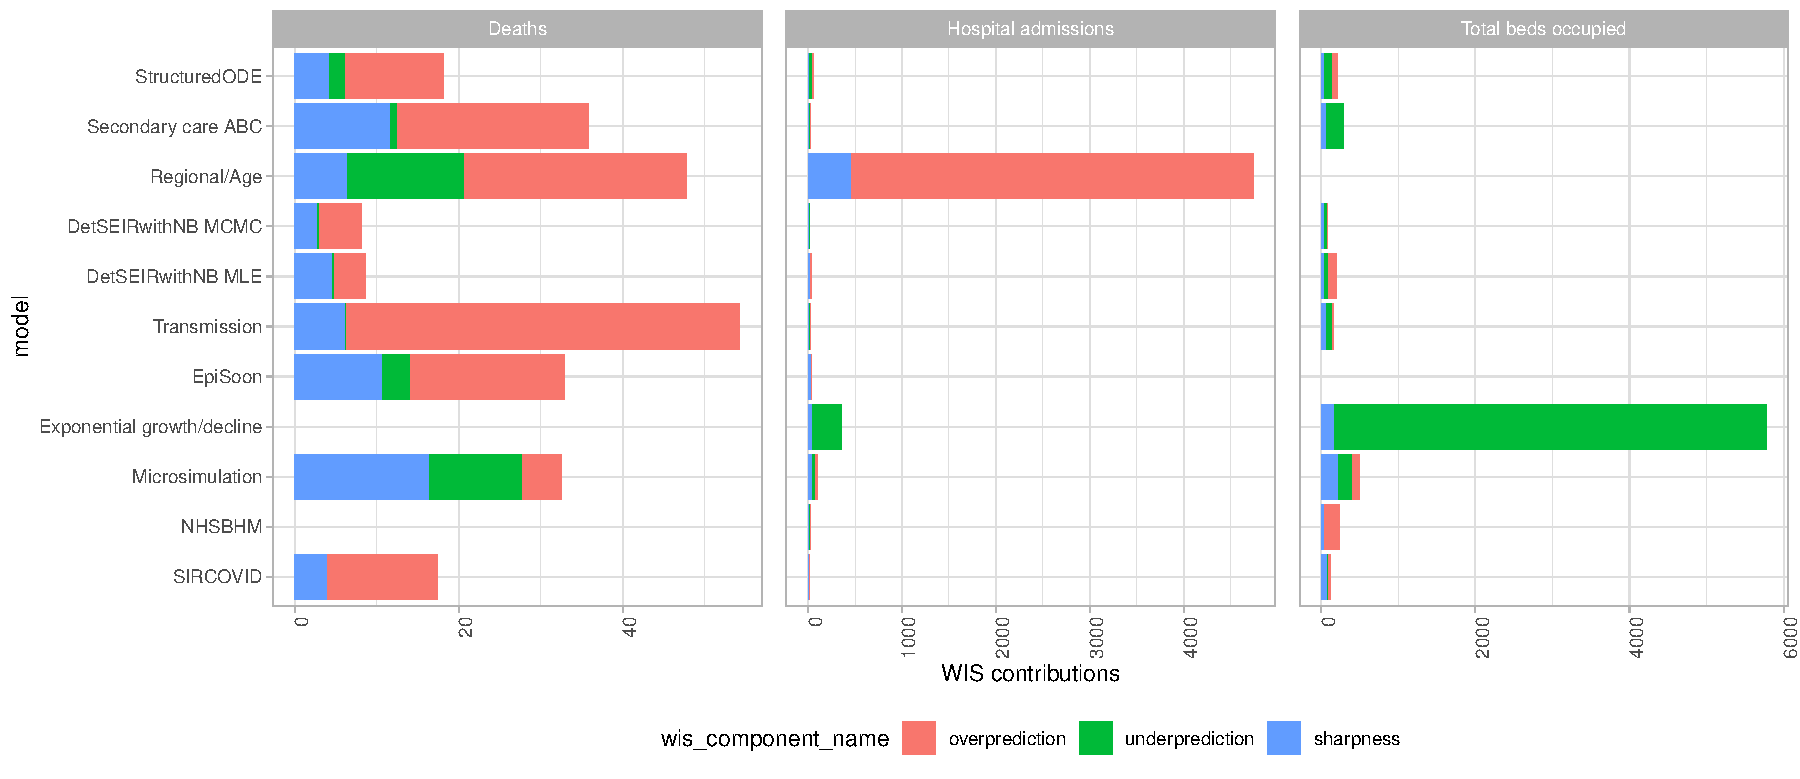
\includegraphics{plots/plot-WIS-components}
\caption{\label{fig:wis-components} p-values and ratios together.}
\end{figure}

We can have a closer look at calibration using the functions \fct{interval\_coverage} and \fct{quantile\_coverage}. The interval coverage plot shows the proportion of all true values that fall within all the different prediction intervals. This gives a visual impression of probabilistic calibration \ref{gneitingProbabilisticForecastsCalibration2007}. Ideally, $x$ percent of true values should be covered by the $x$\%-prediction intervals, resulting in a 45° line. Areas shaded in green indicate that the model is covering more true values than it actually should, while areas in white indicate that the model fails to cover the desired proportion of true values with its prediction intervals. The majority of the models were too confident in their predictions, while some showed showed good calibration. The quantile coverage plot shows the proportion of all true values below certain predictive quantiles. While this plot is slightly harder to interpret, it also includes information about bias as and allows to separate the lower and upper boundaries of the prediction intervals. We can see, for example, that the Exponential growth/decline model was consistently biased downwards. Figure \ref{fig:coverage}

\begin{figure}[h!]
\centering
\begin{Schunk}
\begin{Sinput}
R> cov_scores <- eval_forecasts(combined, 
+                               summarise_by = c("model", 
+                                                "range", "quantile"))
R> scoringutils::interval_coverage(cov_scores)
R> scoringutils::quantile_coverage(cov_scores)
\end{Sinput}
\end{Schunk}
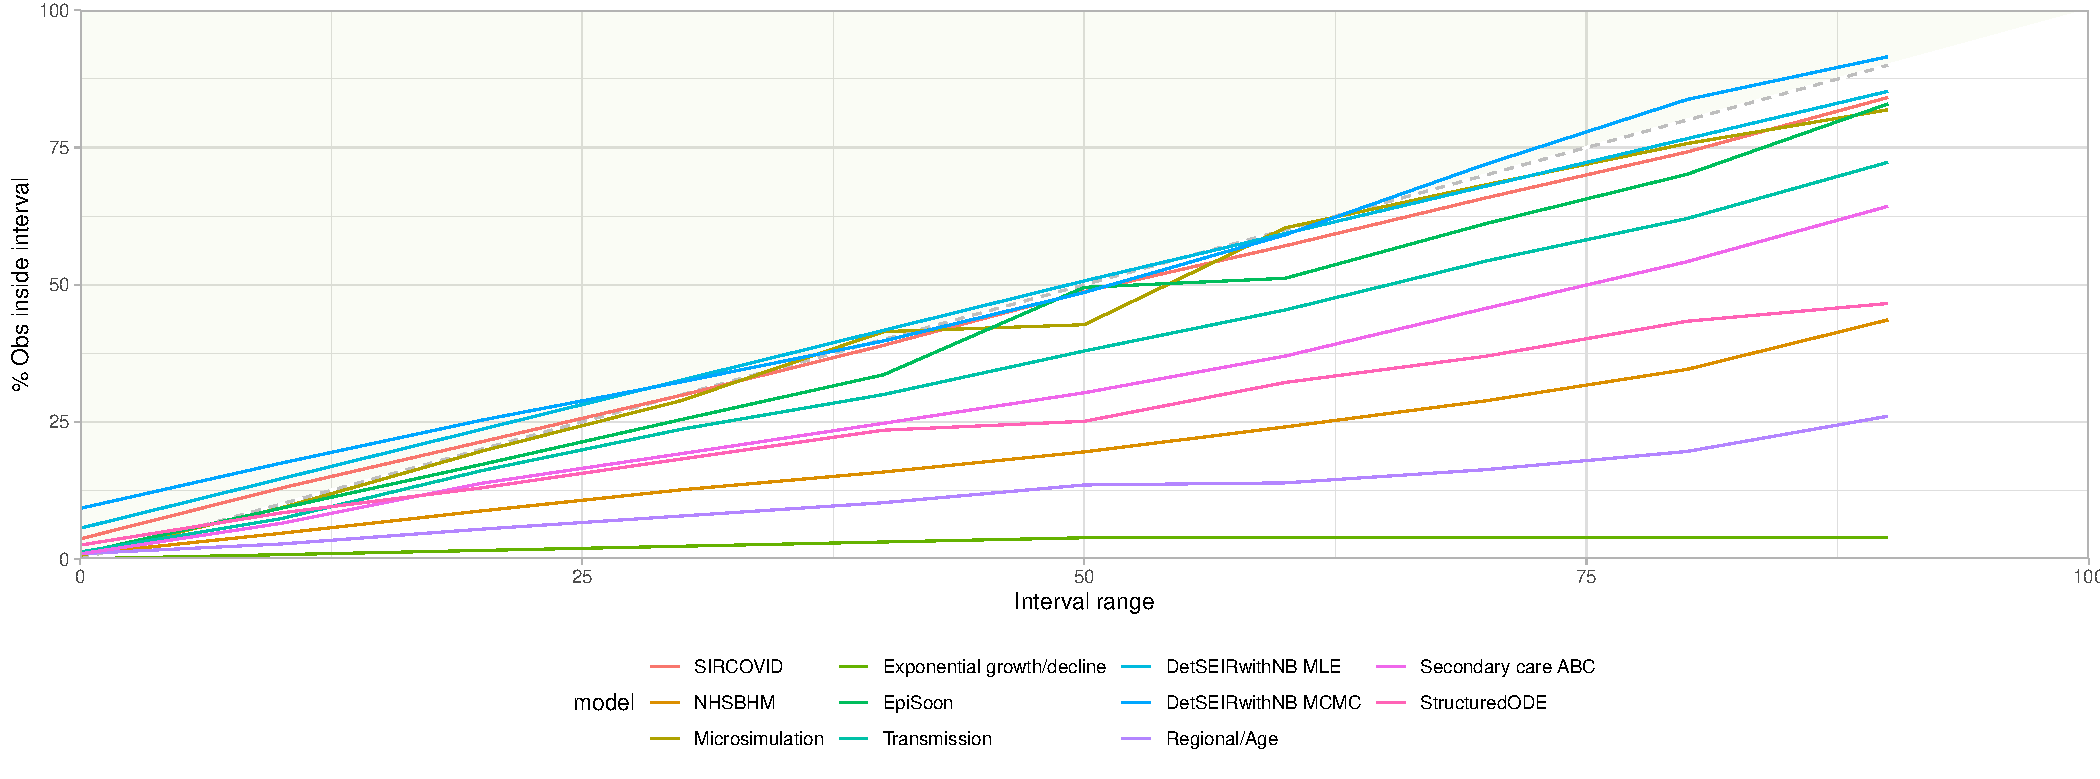
\includegraphics{plots/plot-coverage}

\begin{Schunk}
\begin{Sinput}
R> cov_scores <- eval_forecasts(combined, 
+                               summarise_by = c("model", 
+                                                "range", "quantile"))
R> scoringutils::quantile_coverage(cov_scores)
\end{Sinput}
\end{Schunk}
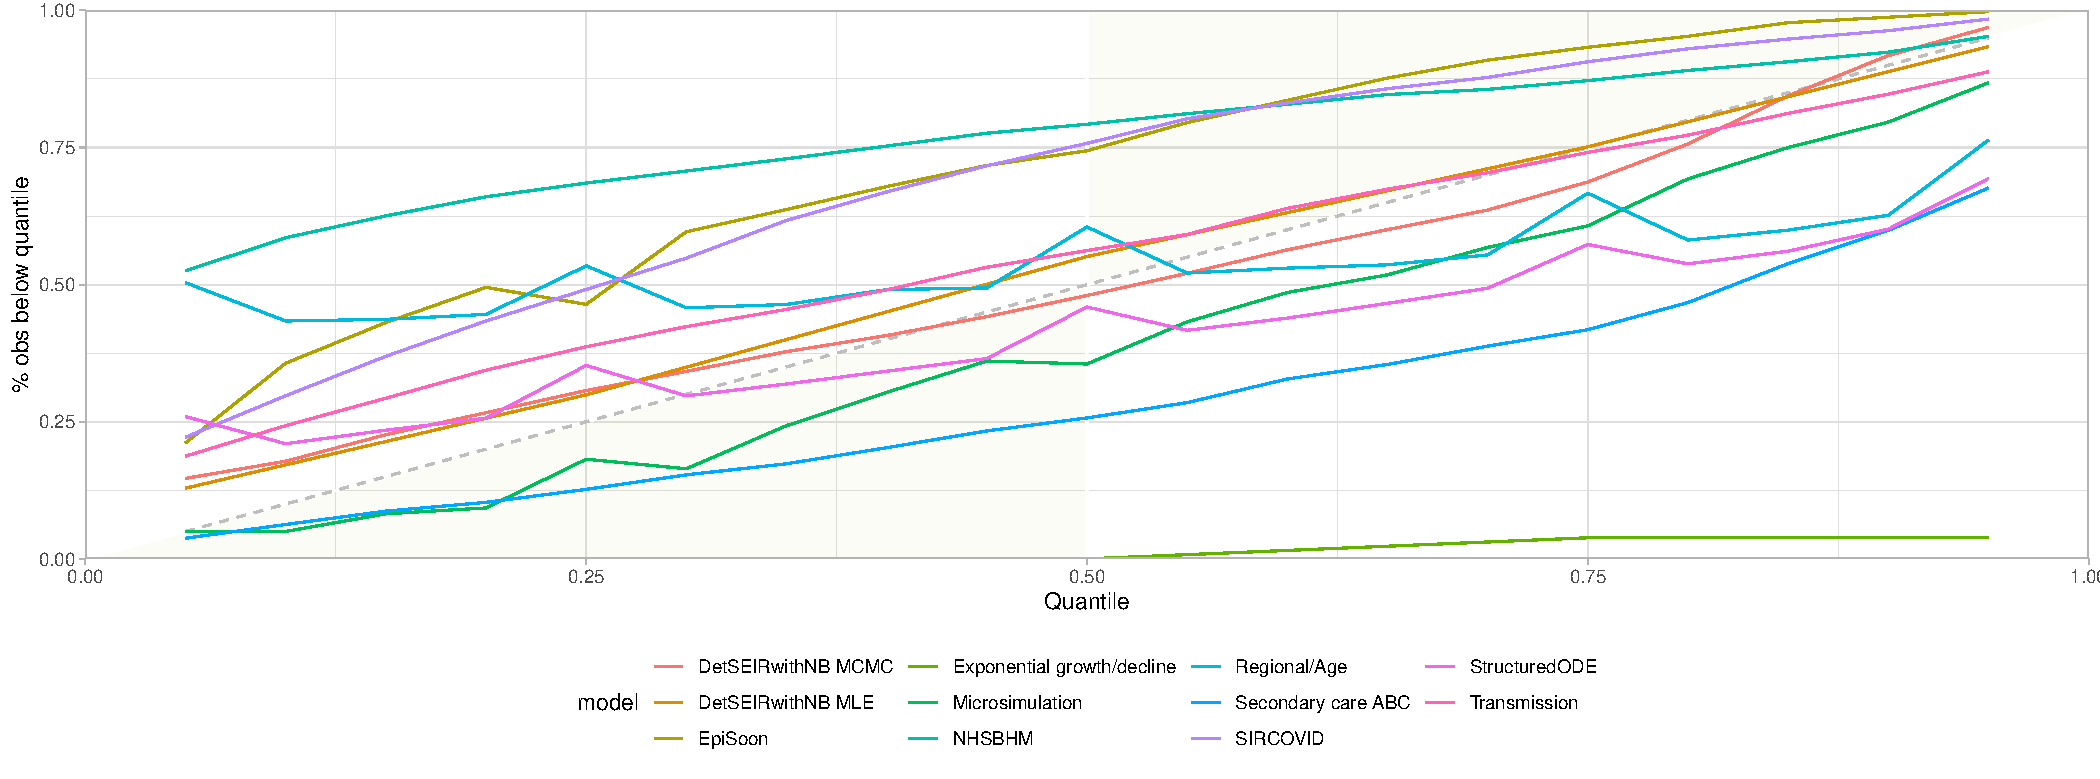
\includegraphics{plots/plot-quantile-coverage}

\caption{\label{fig:coverage} quantile and interval coverage}
\end{figure}


DO I WANT TO INCLUDE PIT PLOTS AS WELL? I GUESS? NEED TO LOOK AT THE IMPLEMENTATION FOR QUANTILE FORECASTS

% \begin{figure}[h]
% \centering
% <<
% pit-plots, echo=TRUE, fig=TRUE, height=5.2, width=12>>=
% # out <- eval_forecasts(combined, 
% #                       summarise_by = c("model"), 
% #                       pit_plots = TRUE)
% 
% @
% \caption{\label{fig:calibration-pit} pit plots}
% \end{figure}

Look at e.g. bias by location? Figure \ref{fig:bias-heatmap}

\begin{figure}[h]
\centering
\begin{Schunk}
\begin{Sinput}
R> scores <- eval_forecasts(combined, 
+                           summarise_by = c("model",
+                                            "value_desc", 
+                                            "geography"), 
+                           compute_relative_skill = FALSE)
R> scoringutils::score_heatmap(scores, metric = "bias", 
+                              x = "geography", facet_formula = ~ value_desc, 
+                              scale = "free_x")
\end{Sinput}
\end{Schunk}
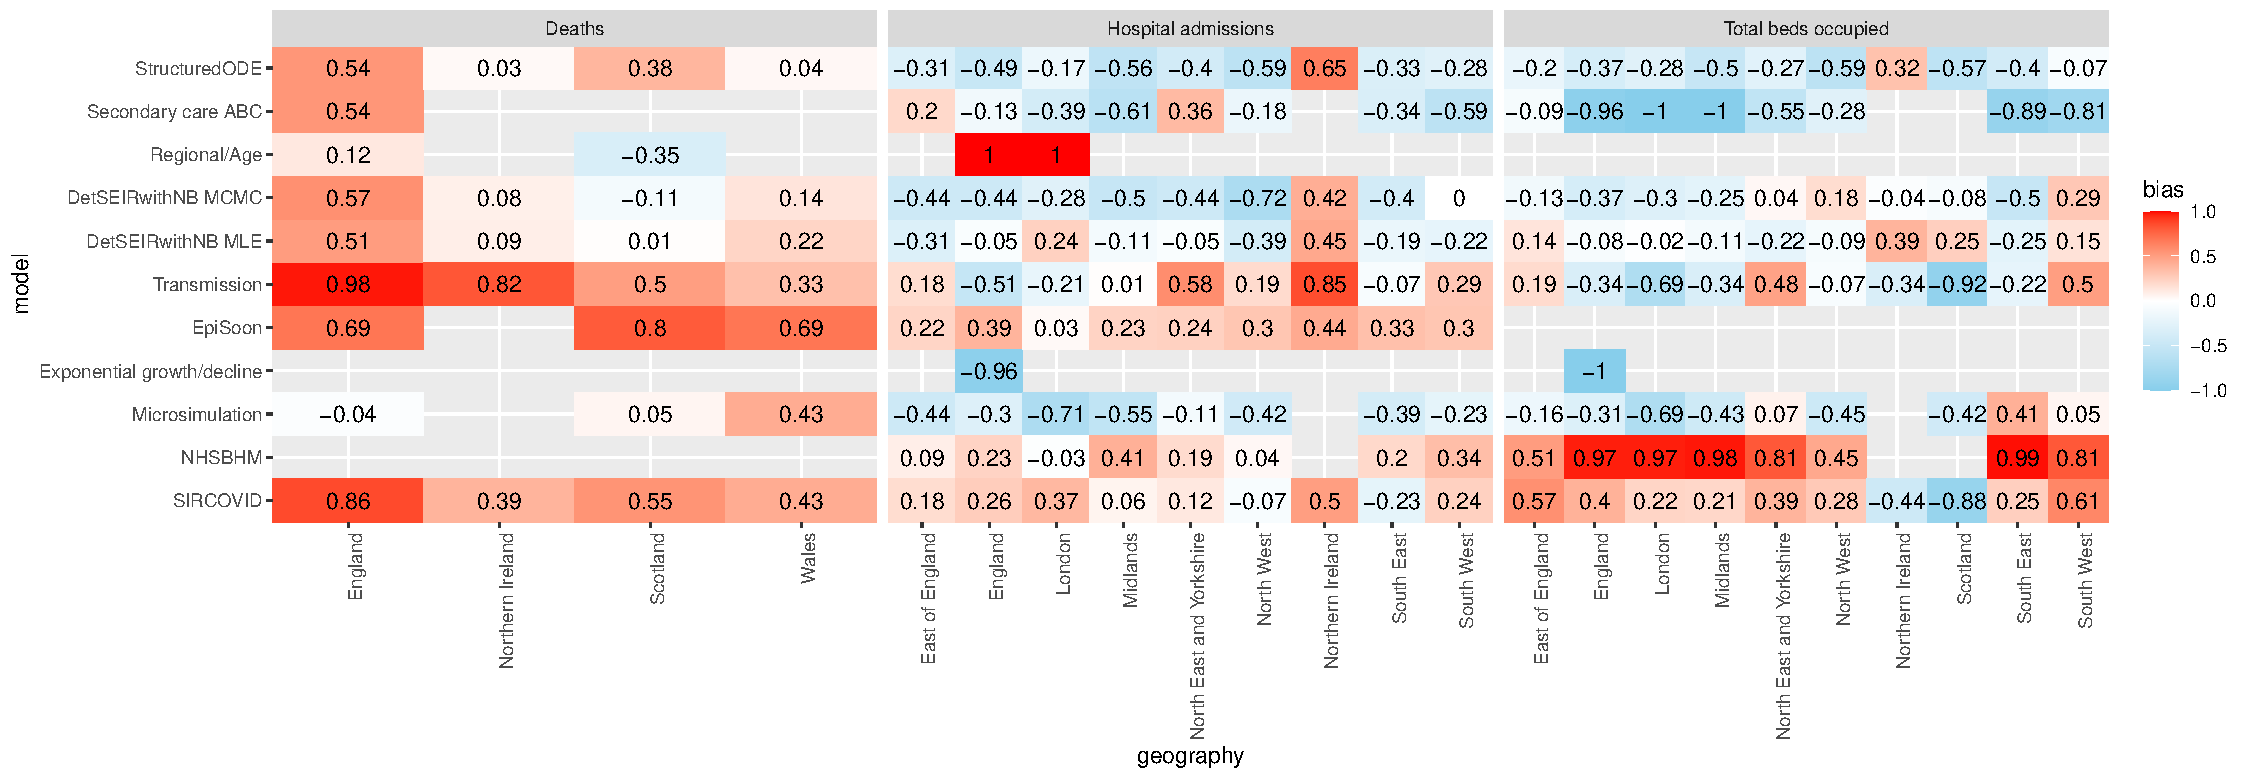
\includegraphics{plots/plot-calibration}
\caption{\label{fig:bias-heatmap} bias by location}
\end{figure}

WHAT IS NEEDED HERE IS A BIT OF THINKING WITH REGARDS TO WHAT VISUALISATION I WANT TO SHOW AND IN HOW MUCH DETAIL I WANT TO ANALYSE THE MODELS. 


\begin{CodeInput}
.
\end{CodeInput}






%% -- Summary/conclusions/discussion -------------------------------------------

\section{Summary and discussion} \label{sec:summary}

COMING SOON. 


% The results in this paper were obtained using
% \proglang{R}~4.0.4 with the
% \pkg{MASS}~7.3.53 package. \proglang{R} itself
% and all packages used are available from the Comprehensive
% \proglang{R} Archive Network (CRAN) at
% \url{https://CRAN.R-project.org/}.


\section*{Acknowledgments}


% All acknowledgments (note the AE spelling) should be collected in this
% unnumbered section before the references. It may contain the usual information
% about funding and feedback from colleagues/reviewers/etc. Furthermore,
% information such as relative contributions of the authors may be added here
% (if any).


%% -- Bibliography -------------------------------------------------------------
%% - References need to be provided in a .bib BibTeX database.
%% - All references should be made with \cite, \citet, \citep, \citealp etc.
%%   (and never hard-coded). See the FAQ for details.
%% - JSS-specific markup (\proglang, \pkg, \code) should be used in the .bib.
%% - Titles in the .bib should be in title case.
%% - DOIs should be included where available.

\bibliography{references}


%% -- Appendix (if any) --------------------------------------------------------
%% - After the bibliography with page break.
%% - With proper section titles and _not_ just "Appendix".

\newpage

\begin{appendix}

\section{Appendix section} \label{app:technical}

\begin{table}[h!]
\centering
\caption{\label{tab:score-table} Explanation of all the scores}
\end{table}


\end{appendix}

%% -----------------------------------------------------------------------------


\end{document}




%BIAS
% For continuous forecasts, assessing whether a predictive distribution has a tendency to over- or underpredict can be very easily achieved by simply evaluating the predictive distribution at the true observed value. This metric is a generalisation of the integer-valued one @funkAssessingPerformanceRealtime2019 have proposed. It is also closely related to the probability integral transform (PIT) discussed later in this chapter. To improve the interpretability of the score we can transform it to a value between -1 (under-prediction) and 1 (over-prediction). Consequently, we measure bias as
% $$B_t (P_t, x_t) = 1 - 2 \cdot (P_t (x_t)),$$
% where $P_t$ is the cumulative distribution function of the predictive distribution for the true value $x_t$. When using predictive samples, $P_t (x_t)$ is simply the fraction of predictive samples for $x_t$ that are smaller than the true observed $x_t$.
% 
% For integer valued forecasts, we use the metric proposed by @funkAssessingPerformanceRealtime2019: 
% $$B_t (P_t, x_t) = 1 - (P_t (x_t) + P_t (x_t + 1)).$$
% Bias can again assume values between -1 (under-prediction) and 1 (over-prediction) and is 0 ideally. 
% 
% For quantile forecasts, we propose the following metric to assess bias: 
% \begin{align*}
%   B_t =& (1 - 2 \cdot \max \{i | q_{t,i} \in Q_t \land q_{t,i} \leq x_t \}) \mathbbm{1}( x_t \leq q_{t, 0.5}) \\
%   &+ (1 - 2 \cdot \min \{i | q_{t,i} \in Q_t \land q_{t,i} \geq x_t\}) \mathbbm{1}( x_t \geq q_{t, 0.5}),
% \end{align*}
% where $Q_t$ is the set of quantiles that form the predictive distribution at time $t$. They represent our belief about what the true value $x_t$ will be. For consistency, we define $Q_t$ such that it always includes the element $q_{t, 0} = - \infty$ and $q_{t,1} = \infty$. $\mathbbm{1}()$ is the indicator function that is $1$ if the condition is satisfied and $0$ otherwise. In clearer terms, $B_t$ is defined as the maximum percentile rank for which the corresponding quantile is still below the true value, if the true value is smaller than the median of the predictive distribution. If the true value is above the median of the predictive distribution, then $B_t$ is the minimum percentile rank for which the corresponding quantile is still larger than the true value. If the true value is exactly the median, both terms cancel out and $B_t$ is zero. For a large enough number of quantiles, the percentile rank will equal the proportion of predictive samples below the observed true value, and this metric coincides with the one for continuous forecasts. 
